\chapter{ODG, dynamic, CGP and ACGP compared on nine benchmarks}
\label{ch:four-policies}

Chapter~\ref{ch:exp1} compared on-demand generation (ODG) and dynamic compiler pre-generation. This chapter adds the two autonomous protocols that the compiler-driven approach is meant to
improve on: CGP (continuous generation, neighbour drawn uniformly) and ACGP (adaptive continuous generation, neighbour probabilities adapted to recent traffic). The goal
stated for the compiler-driven approach is a latency comparable to the alternatives with fewer wasted pairs, so the comparison is on latency, delivered fidelity, wasted pairs and readiness, with the
wait for a free memory as the explanation.

\section{What was run}
Same traces, memory counts ($2,3,4,6,8,16,32$; QFT also $64$), mapping seeds (42, 43, 44), physics seeds (0, 1, 2), physical parameters and corrected scheduler as Experiment~1, on the mesh and on the
torus, for CGP and for ACGP: $384$ invocations ($1\,152$ runs) per topology. ODG and dynamic are the Experiment~1 runs, not repeated. Two settings of the autonomous protocols needed a decision and were made so that the
comparison with dynamic is fair, as opt-in options that leave the default behaviour untouched (the 164-row legacy baseline still reproduces exactly, and all 162 tests pass):
\begin{itemize}
  \item \textbf{Cache cap.} ACE's configuration file gives the autonomous protocols a fixed cap of three cached pairs per core whatever the number of memories (\code{adaptive_max_memory}). Dynamic is given a compiler bank of memories$-1$.
    CGP and ACGP are given the same cap, memories$-1$ (\code{--autonomous-cache-follows-compiler-memories}). With the fixed cap of three they would have been allowed to cache three pairs in two memories.
  \item \textbf{End of the run.} The autonomous protocols keep generating pairs until the simulation's stop time (300\,s of simulated time), long after the last request. The runs were stopped 1\,ms after the last request completed
    (\code{--stop-after-workload}), so that wasted pairs are counted over the workload's own duration and not over an arbitrary stop time. This changes no request metric: for QFT at four memories CGP's latency is
    $9.963931$\,ms with and without it.
\end{itemize}
The \textbf{random circuit was set aside} for CGP and ACGP: its runs at large memory counts take over an hour each. It is therefore left out of every table and figure in this chapter (ODG and dynamic for it are in Chapter~\ref{ch:exp1};
the diagnostic Table~\ref{tab:diag-workloads} has all four policies for it at four memories, mapping seed 42). The runs that had finished when it was stopped are kept in the results folder but not analysed.

\paragraph{Definitions.} Latency is the common latency of Chapter~\ref{ch:corrections}. \emph{Wait} is the part of it spent waiting for a free memory. \emph{Waste} is $(\text{pairs generated}-\text{pairs used})/\text{pairs generated}$ from the
simulator's protocol counters over the workload's duration; a pair still cached when the run stops counts as not used, as in the compiler's own accounting. (The simulator's own waste figure counts only pairs that expired unused and
is lower for short workloads; both are in \code{four_policy_cell_means.csv}.) \emph{Readiness} is pairs used per request: for dynamic it equals the share of requests served from a ready pair; for CGP and ACGP it is the number of
cached pairs that requests consumed, divided by the number of requests (a pair is counted at both of its endpoints, so the counters are divided by twice the number of requests).

\section{Checks}
\begin{itemize}
  \item Every one of the $2\,304$ CGP/ACGP runs ($1\,152$ per topology) completed every request (completion rate $1.0$).
  \item The waste counters were checked against an independent count of the pair events on one run (QFT, four memories, CGP): $4\,720$ pairs generated and $3\,068$ used by both counts. The simulator's ``unused'' counter, which is
    incremented when a cached memory is released, agreed with the count of pairs that expired while cached to within $1.2\%$ (it also counts $20$ releases of memories that held no pair).
  \item Dynamic's compiler pairs were all used in every one of the $639$ mesh runs of Experiment~1 (none expired, none left over); on the torus at most one pair expired in any of its $639$ runs (at most $0.013\%$ of a run's pairs).
  \item The mechanism behind every number was read in the code and measured separately (Chapter~\ref{ch:why-dynamic}).
\end{itemize}

\section{Latency}
\begin{landscape}
\begin{figure}[p]
\centering
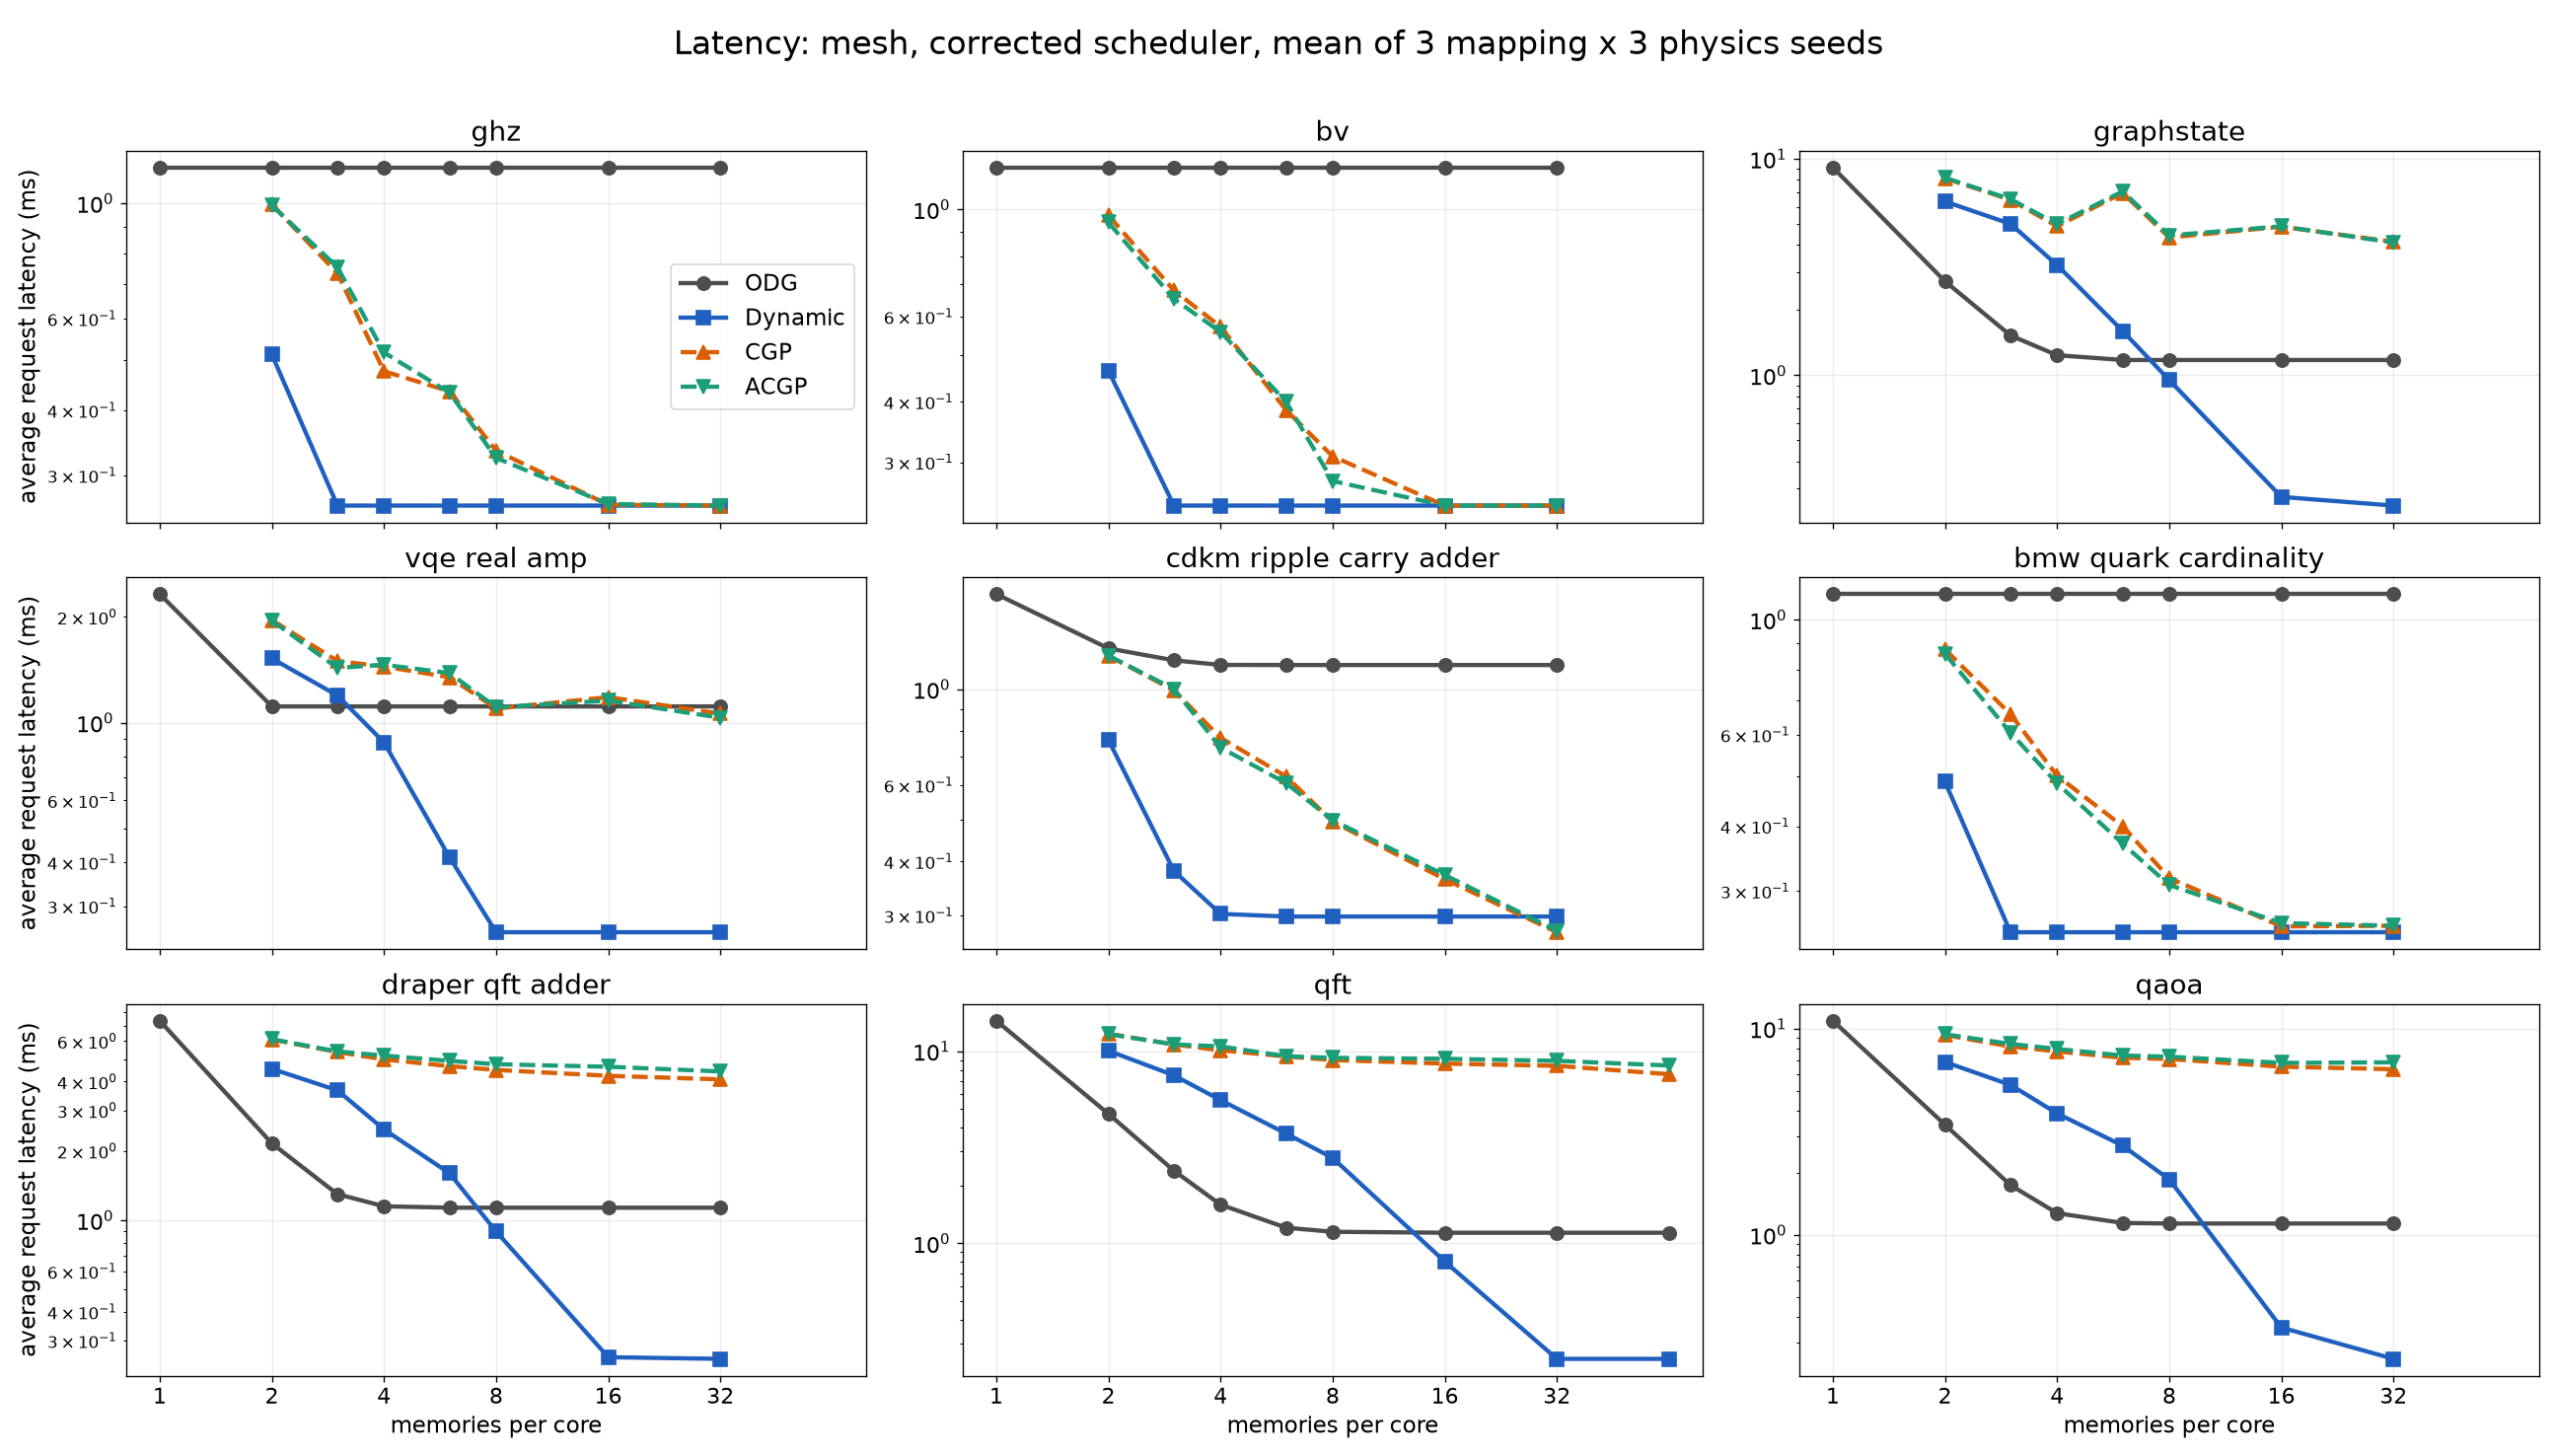
\includegraphics[width=\linewidth,height=0.80\textheight,keepaspectratio]{fp_mesh_latency.png}
\caption{Request latency against memories per core, all four policies (log scale). Mesh, corrected scheduler, mean of three mapping seeds of the mean of three physics seeds; CGP and ACGP cache at most memories$-1$ pairs per core.}
\label{fig:fp-mesh-lat}
\end{figure}
\end{landscape}

\begin{table}[H]
\centering\small
\resizebox{\ifdim\width>\linewidth\linewidth\else\width\fi}{!}{%
\begin{tabular}{@{}lrrrr@{}}
\toprule
Workload & ODG & Dynamic & CGP & ACGP \\
\midrule
GHZ & 1.17 & 0.26 & 0.48 & 0.52 \\
Bernstein--Vazirani & 1.22 & 0.24 & 0.57 & 0.56 \\
BMW/QUARK cardinality & 1.12 & 0.25 & 0.50 & 0.48 \\
VQE real amplitudes & 1.11 & 0.88 & 1.44 & 1.46 \\
CDKM ripple-carry adder & 1.14 & 0.30 & 0.77 & 0.73 \\
Graph state & 1.24 & 3.23 & 4.88 & 5.00 \\
Draper QFT adder & 1.15 & 2.48 & 5.00 & 5.19 \\
QAOA & 1.27 & 3.88 & 7.75 & 7.97 \\
QFT & 1.59 & 5.57 & 10.11 & 10.60 \\
\bottomrule
\end{tabular}}
\caption{Request latency (ms), mesh, 4 memories per core (modelled), mean of three mapping seeds of the mean of three physics seeds.}
\label{tab:fp-mesh-lat-4}
\end{table}

Figure~\ref{fig:fp-mesh-lat} and Table~\ref{tab:fp-mesh-lat-4} give the picture on the mesh. Three results stand out.
\begin{itemize}
  \item \textbf{Dynamic is the fastest of the three pre-generation policies at every memory count from two on, on every benchmark} except one cell (CDKM adder at $32$ memories, where CGP and ACGP are $0.27$ against dynamic's $0.30$\,ms; Table~\ref{tab:fp-mesh-where}).
    At four memories the better of CGP and ACGP takes $1.5$ to $2.4$ times dynamic's latency on the mesh and $1.9$ to $2.5$ times on the torus.
  \item \textbf{Against ODG, dynamic wins on five of the nine benchmarks at the modelled four memories and loses on four.} It wins on BMW, Bernstein--Vazirani, GHZ, the CDKM adder and VQE, and at $32$ memories it is $74$ to $80\%$ faster than ODG on all nine
    (ODG's floor is the generation time of about a millisecond, a ready pair needs a quarter of that); on four of the five it is faster from two memories on.
    It loses on QFT, QAOA, Draper and graph state at two to four memories and overtakes ODG from eight memories on Draper and graph state and from sixteen on QAOA and QFT (Tables~\ref{tab:fp-mesh-gain} and~\ref{tab:fp-mesh-where}).
    The cause is Chapter~\ref{ch:why-dynamic}.
  \item \textbf{CGP and ACGP beat ODG only where ODG is already at its floor.} They are faster than ODG at every memory count on BMW, Bernstein--Vazirani, GHZ and the CDKM adder, and on VQE at some, but \emph{never} on QFT, QAOA, Draper or graph state: at four memories
    they take $4.9$ to $10.6$\,ms on those four against $1.2$ to $1.6$\,ms for ODG. Their wait barely improves with memory.
\end{itemize}
ACGP is not measurably better than CGP: their latencies differ by a median of $2.5\%$ on the mesh and $1.9\%$ on the torus (at most $11\%$ and $14\%$), and their waste by under two points. Why the adaptation has so little effect was not investigated.
\begin{table}[H]
\centering\small
\resizebox{\ifdim\width>\linewidth\linewidth\else\width\fi}{!}{%
\begin{tabular}{@{}lrrrr@{}}
\toprule
Workload & ODG & Dynamic & CGP & ACGP \\
\midrule
GHZ & 1.17 & 0.51 & 1.00 & 0.99 \\
Bernstein--Vazirani & 1.22 & 0.46 & 0.97 & 0.94 \\
BMW/QUARK cardinality & 1.12 & 0.49 & 0.88 & 0.86 \\
VQE real amplitudes & 1.11 & 1.52 & 1.96 & 1.95 \\
CDKM ripple-carry adder & 1.24 & 0.76 & 1.19 & 1.20 \\
Graph state & 2.72 & 6.36 & 8.15 & 8.19 \\
Draper QFT adder & 2.16 & 4.55 & 6.10 & 6.11 \\
QAOA & 3.42 & 6.89 & 9.31 & 9.39 \\
QFT & 4.72 & 10.06 & 12.34 & 12.27 \\
\bottomrule
\end{tabular}}
\caption{Request latency (ms), mesh, 2 memories per core (modelled), mean of three mapping seeds of the mean of three physics seeds.}
\label{tab:fp-mesh-lat-2}
\end{table}

\begin{table}[H]
\centering\small
\resizebox{\ifdim\width>\linewidth\linewidth\else\width\fi}{!}{%
\begin{tabular}{@{}lrrrrrrr@{}}
\toprule
Workload & 2 & 3 & 4 & 6$^*$ & 8$^*$ & 16$^*$ & 32$^*$ \\
\midrule
GHZ & 56\% & 78\% & 78\% & 78\% & 78\% & 78\% & 78\% \\
Bernstein--Vazirani & 62\% & 80\% & 80\% & 80\% & 80\% & 80\% & 80\% \\
BMW/QUARK cardinality & 56\% & 78\% & 78\% & 78\% & 78\% & 78\% & 78\% \\
VQE real amplitudes & -37\% & -7\% & 21\% & 63\% & 77\% & 77\% & 77\% \\
CDKM ripple-carry adder & 39\% & 67\% & 73\% & 74\% & 74\% & 74\% & 74\% \\
Graph state & -134\% & -228\% & -161\% & -36\% & 19\% & 77\% & 79\% \\
Draper QFT adder & -111\% & -182\% & -116\% & -41\% & 21\% & 78\% & 78\% \\
QAOA & -101\% & -207\% & -205\% & -137\% & -64\% & 69\% & 78\% \\
QFT & -113\% & -214\% & -250\% & -209\% & -142\% & 29\% & 78\% \\
Random circuit & -51\% & -22\% & 15\% & 50\% & 66\% & 77\% & 77\% \\
\bottomrule
\end{tabular}}
\caption{Latency gain of dynamic over on-demand, $(\text{ODG}-\text{Dyn.})/\text{ODG}$, mesh; negative means dynamic is slower. Budgets marked $^*$ are counterfactual.}
\label{tab:fp-mesh-gain}
\end{table}

\begin{table}[H]
\centering\small
\resizebox{\ifdim\width>\linewidth\linewidth\else\width\fi}{!}{%
\begin{tabular}{@{}lcccrrrr@{}}
\toprule
Workload & Dynamic beats ODG from (memories) & vs CGP win/tie/loss & vs ACGP win/tie/loss & Fidelity Dyn. & CGP & ACGP & ODG \\
\midrule
GHZ & 2 & 6/1/0 & 6/1/0 & 0.925 & 0.877 & 0.878 & 0.950 \\
Bernstein--Vazirani & 2 & 5/2/0 & 5/2/0 & 0.927 & 0.868 & 0.865 & 0.950 \\
BMW/QUARK cardinality & 2 & 7/0/0 & 7/0/0 & 0.925 & 0.872 & 0.870 & 0.950 \\
VQE real amplitudes & 4 & 7/0/0 & 7/0/0 & 0.916 & 0.899 & 0.899 & 0.950 \\
CDKM ripple-carry adder & 2 & 6/0/1 & 6/0/1 & 0.923 & 0.913 & 0.912 & 0.950 \\
Graph state & 8 & 7/0/0 & 7/0/0 & 0.919 & 0.900 & 0.900 & 0.950 \\
Draper QFT adder & 8 & 7/0/0 & 7/0/0 & 0.922 & 0.903 & 0.902 & 0.950 \\
QAOA & 16 & 7/0/0 & 7/0/0 & 0.925 & 0.905 & 0.904 & 0.950 \\
QFT & 16 & 8/0/0 & 8/0/0 & 0.927 & 0.908 & 0.905 & 0.950 \\
Random circuit & 4 & 6/0/0 & 5/0/0 & 0.913 & 0.899 & 0.898 & 0.950 \\
\bottomrule
\end{tabular}}
\caption{Where dynamic lies, mesh. Column~2: the smallest memory count from which dynamic has lower latency than on-demand ($^\dagger$: with at least one later count where it does not). Columns~3--4: over the memory counts run for both policies (2 to 32; QFT also 64), the number at which dynamic has lower latency, equal latency (the floor reached when nothing waits) or higher latency than CGP and than ACGP. Columns~5--8: delivered fidelity at four memories.}
\label{tab:fp-mesh-where}
\end{table}

\begin{table}[H]
\centering\small
\resizebox{\ifdim\width>\linewidth\linewidth\else\width\fi}{!}{%
\begin{tabular}{@{}rrrrr@{}}
\toprule
Mem. & ODG & Dynamic & CGP & ACGP \\
\midrule
1 & 9 & 0 & 0 & 0 \\
2 & 5 & 4 & 0 & 0 \\
3 & 5 & 4 & 0 & 0 \\
4 & 4 & 5 & 0 & 0 \\
6 & 4 & 5 & 0 & 0 \\
8 & 2 & 7 & 0 & 0 \\
16 & 0 & 8 & 0 & 1 \\
32 & 0 & 6 & 1 & 2 \\
\bottomrule
\end{tabular}}
\caption{Mesh: number of benchmarks (of ten) on which each policy has the lowest latency at each memory count (a policy is counted only where it was run; dynamic, CGP and ACGP start at two memories).}
\label{tab:fp-mesh-best}
\end{table}


\section{Delivered fidelity}
\clearpage\newgeometry{margin=12mm}\begin{landscape}
\begin{figure}[p]
\centering
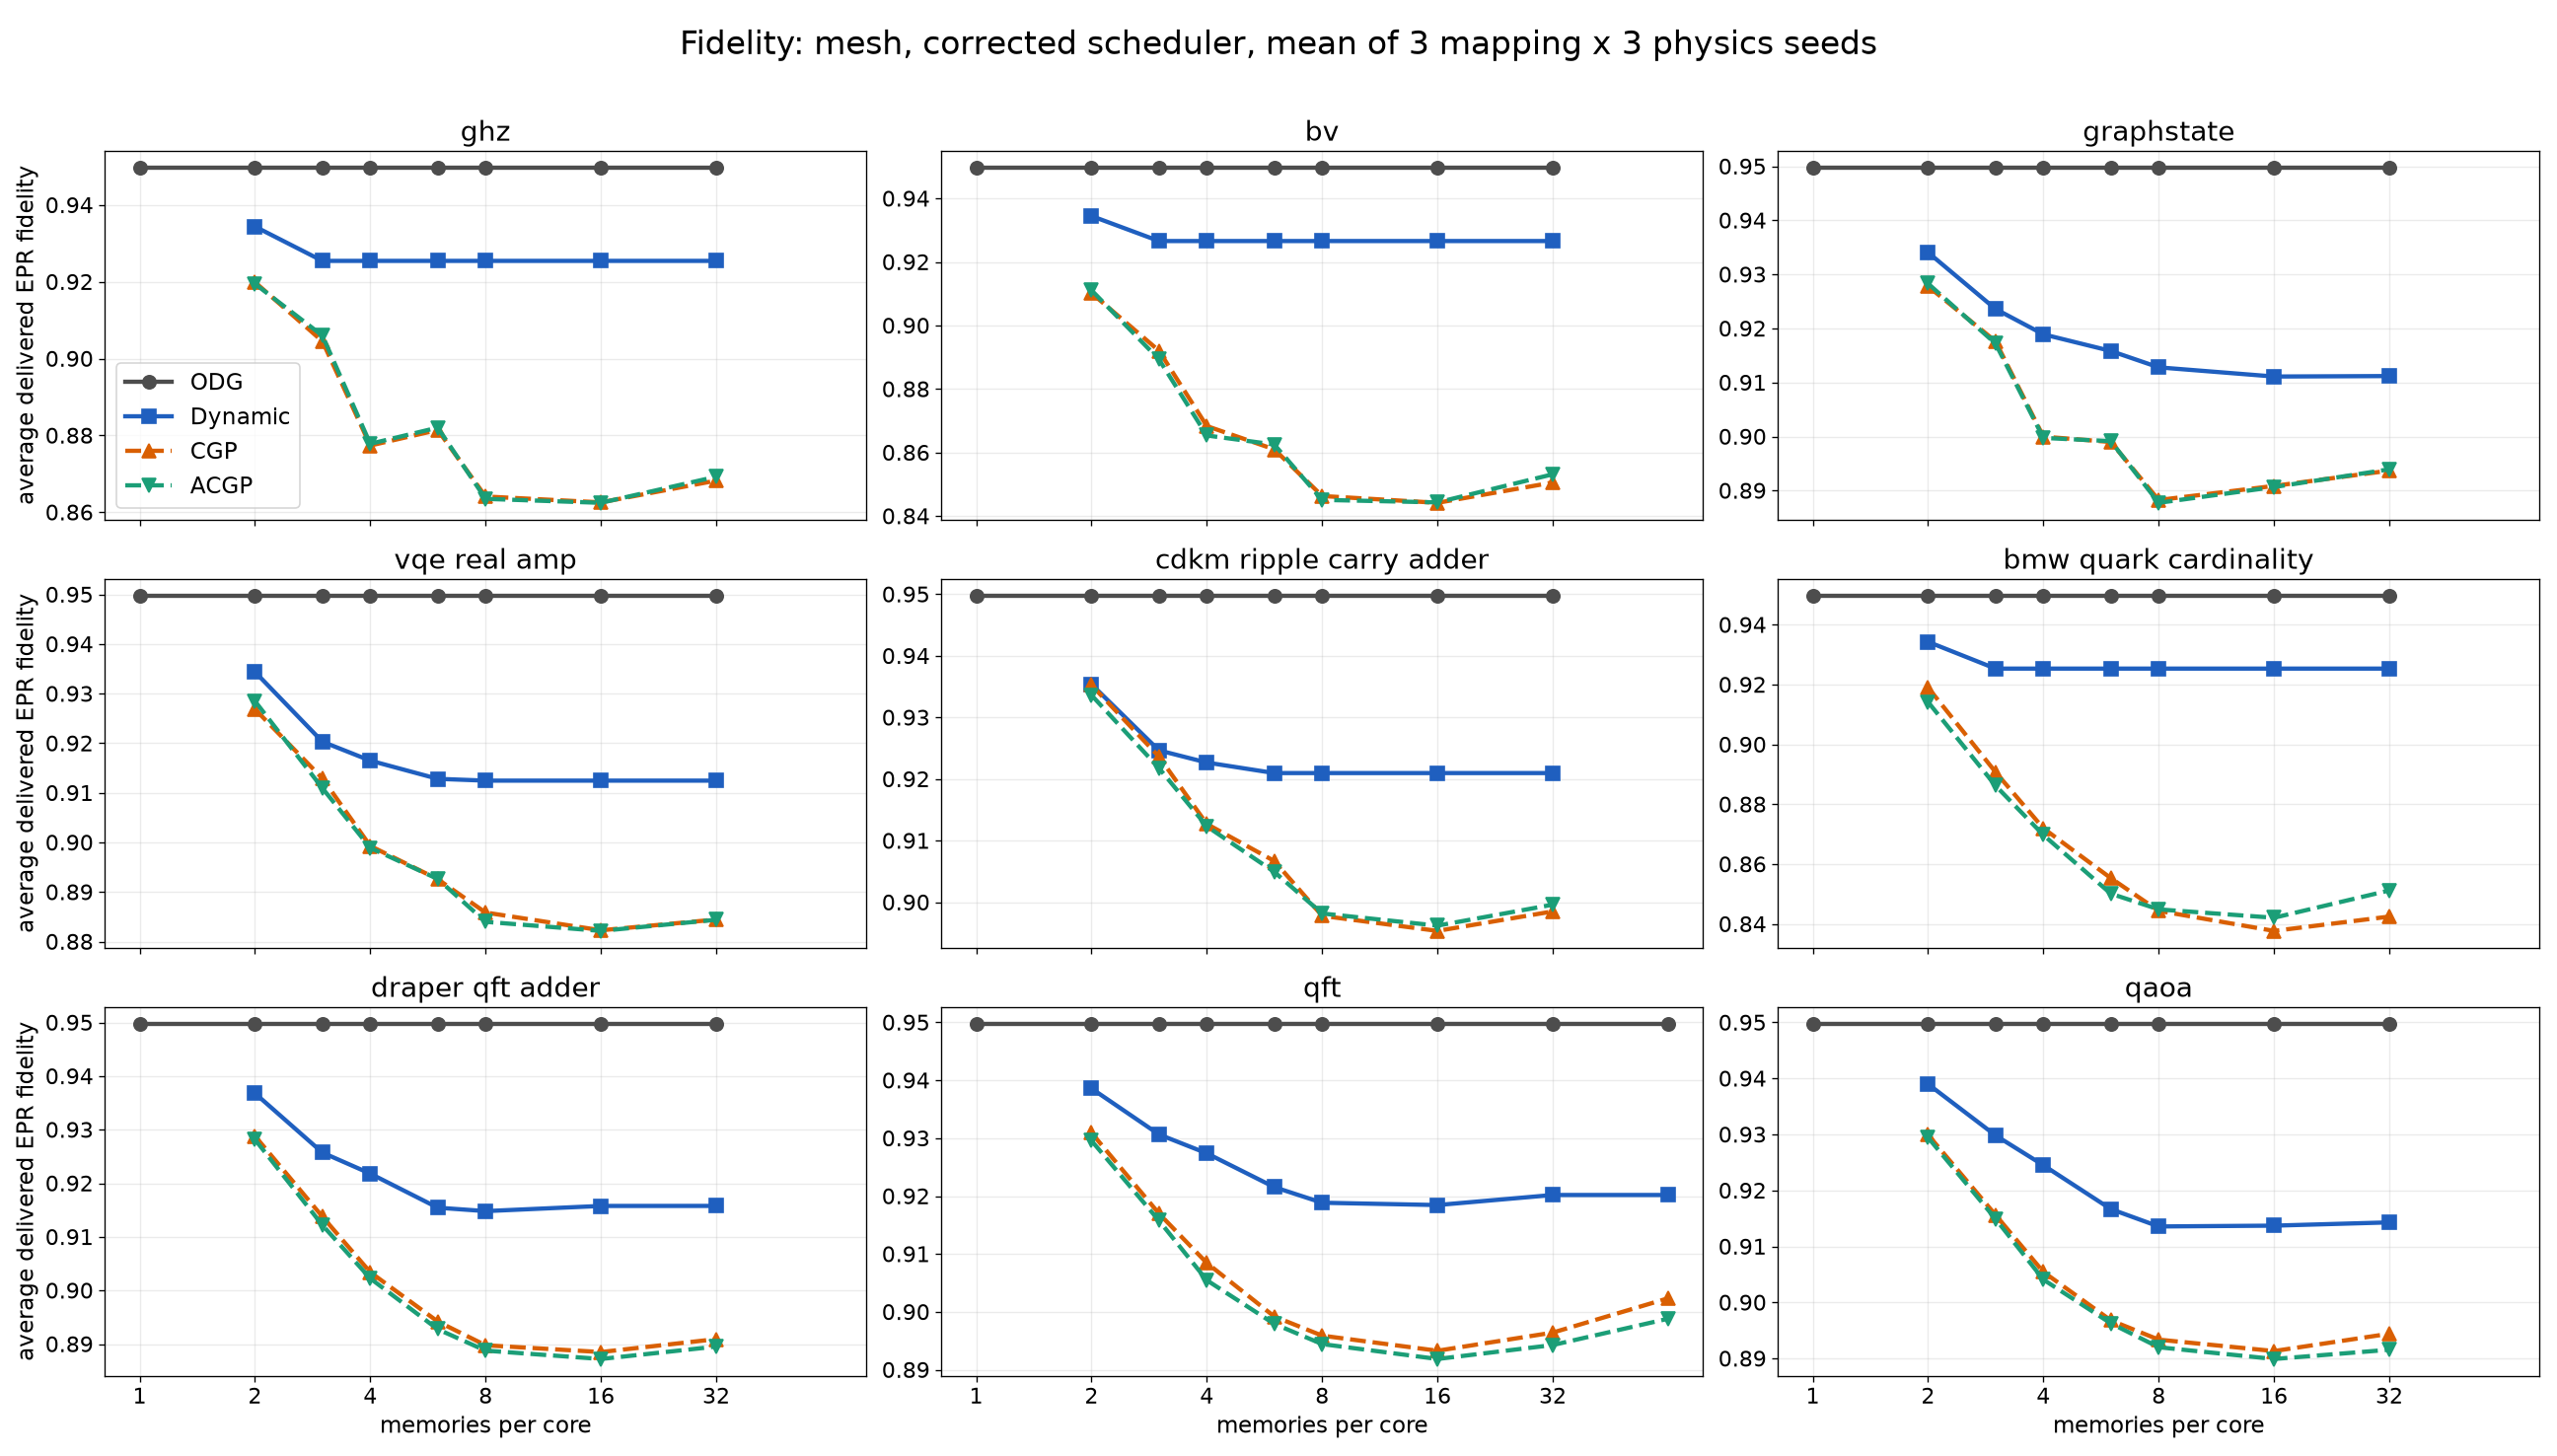
\includegraphics[width=\linewidth,height=0.82\textheight,keepaspectratio]{fp_mesh_fidelity.png}
\caption{Delivered EPR fidelity against memories per core. Mesh, corrected scheduler, mean of three mapping seeds of the mean of three physics seeds; CGP and ACGP cache at most memories$-1$ pairs per core.}
\label{fig:fp-mesh-fid}
\end{figure}
\end{landscape}\clearpage\restoregeometry

\begin{table}[H]
\centering\small
\resizebox{\ifdim\width>\linewidth\linewidth\else\width\fi}{!}{%
\begin{tabular}{@{}lrrrr@{}}
\toprule
Workload & ODG & Dynamic & CGP & ACGP \\
\midrule
GHZ & 0.9498 & 0.9254 & 0.8774 & 0.8778 \\
Bernstein--Vazirani & 0.9498 & 0.9266 & 0.8683 & 0.8654 \\
BMW/QUARK cardinality & 0.9498 & 0.9253 & 0.8720 & 0.8697 \\
VQE real amplitudes & 0.9498 & 0.9165 & 0.8993 & 0.8989 \\
CDKM ripple-carry adder & 0.9498 & 0.9227 & 0.9127 & 0.9123 \\
Graph state & 0.9498 & 0.9189 & 0.9000 & 0.8997 \\
Draper QFT adder & 0.9498 & 0.9218 & 0.9034 & 0.9022 \\
QAOA & 0.9498 & 0.9245 & 0.9054 & 0.9041 \\
QFT & 0.9498 & 0.9274 & 0.9084 & 0.9055 \\
Random circuit & 0.9498 & 0.9130 & 0.8989 & 0.8976 \\
\bottomrule
\end{tabular}}
\caption{Delivered EPR fidelity, mesh, 4 memories per core (modelled), mean of three mapping seeds of the mean of three physics seeds.}
\label{tab:fp-mesh-fid-4}
\end{table}

ODG delivers $0.950$ always. Dynamic's pairs wait in memory and decohere: its fidelity is $0.911$ to $0.939$ over all budgets ($0.916$ to $0.927$ at four memories) and falls from two to $32$ memories on every benchmark, as the compiler bank grows. CGP and ACGP are lower and more
variable, $0.838$ to $0.935$ over all budgets ($0.865$ to $0.913$ at four memories), presumably because their pairs age longer before use (the age of CGP and ACGP pairs was not measured). Dynamic's pairs are
better by $0.01$ to $0.06$ at four memories, but never as good as on-demand pairs. (These figures use ACE's coherence time of one second; under the group's multi-core paper's $1$\,ms every cached pair would expire, Chapter~\ref{ch:exp1}.)

\section{Wasted pairs and readiness}
\clearpage\newgeometry{margin=12mm}\begin{landscape}
\begin{figure}[p]
\centering
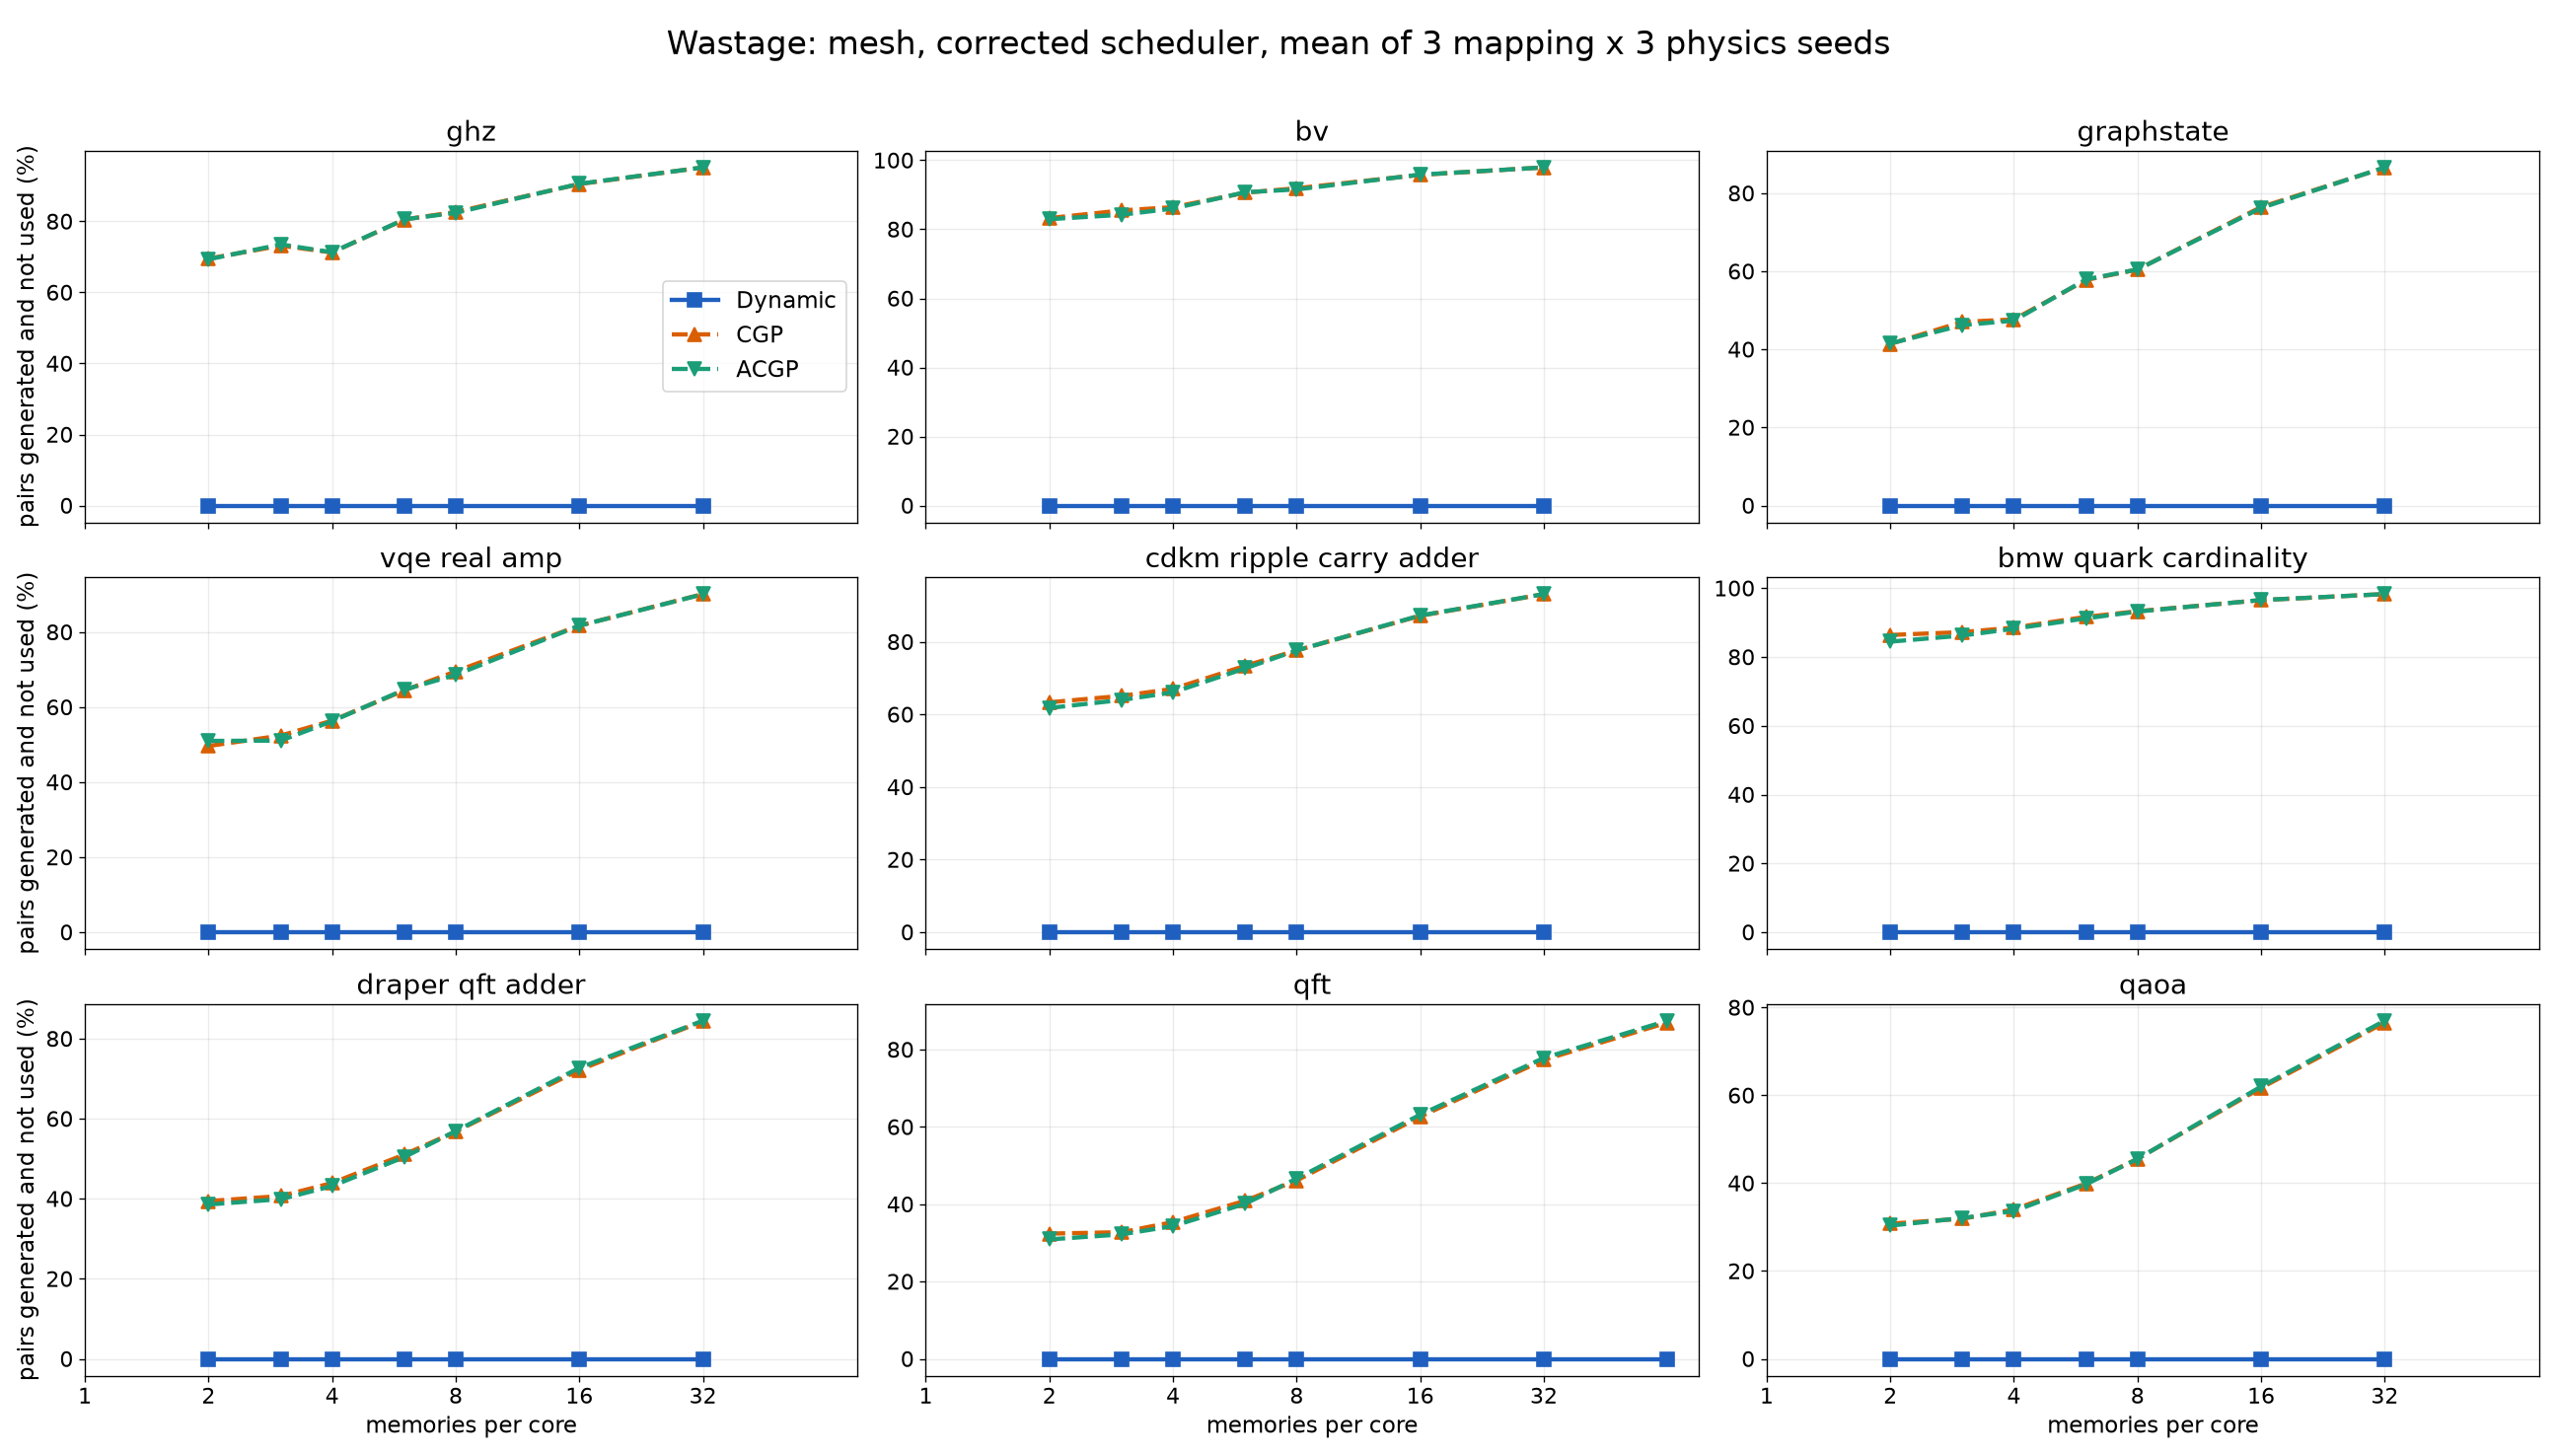
\includegraphics[width=\linewidth,height=0.82\textheight,keepaspectratio]{fp_mesh_waste.png}
\caption{Pairs generated and not used by the end of the run, as a percentage of pairs generated (dynamic, CGP, ACGP). Mesh, corrected scheduler, mean of three mapping seeds of the mean of three physics seeds; CGP and ACGP cache at most memories$-1$ pairs per core.}
\label{fig:fp-mesh-waste}
\end{figure}
\end{landscape}\clearpage\restoregeometry

\begin{table}[H]
\centering\small
\resizebox{\ifdim\width>\linewidth\linewidth\else\width\fi}{!}{%
\begin{tabular}{@{}lrrr@{}}
\toprule
Workload & Dynamic & CGP & ACGP \\
\midrule
GHZ & 0.0 & 71.3 & 71.3 \\
Bernstein--Vazirani & 0.0 & 86.4 & 86.0 \\
BMW/QUARK cardinality & 0.0 & 88.6 & 88.2 \\
VQE real amplitudes & 0.0 & 56.4 & 56.3 \\
CDKM ripple-carry adder & 0.0 & 67.1 & 66.1 \\
Graph state & 0.0 & 47.7 & 47.4 \\
Draper QFT adder & 0.0 & 43.9 & 43.2 \\
QAOA & 0.0 & 34.0 & 33.6 \\
QFT & 0.0 & 35.4 & 34.3 \\
\bottomrule
\end{tabular}}
\caption{Pairs generated and never used (\%), mesh, 4 memories per core (modelled), mean of three mapping seeds of the mean of three physics seeds.}
\label{tab:fp-mesh-waste-4}
\end{table}

Dynamic wastes no pair on the mesh (every prepared pair is used). CGP and ACGP waste $34$ to $89\%$ of their pairs at four memories on the mesh, and more with more memory
($31\%$ on QFT at two memories, $78\%$ at $32$): they make pairs for neighbours drawn at random, and a pair nobody uses before its window ends is lost. The percentage depends on the size of the workload: at four memories it is highest on BMW, Bernstein--Vazirani, GHZ
and the CDKM adder ($24$ to $456$ requests) and lowest on QAOA, QFT and Draper ($1\,310$ to $3\,068$ requests), so it is comparable only within a benchmark. Cached pairs, used or not, are also what block requests (Chapter~\ref{ch:why-dynamic}).
\begin{landscape}
\begin{figure}[p]
\centering
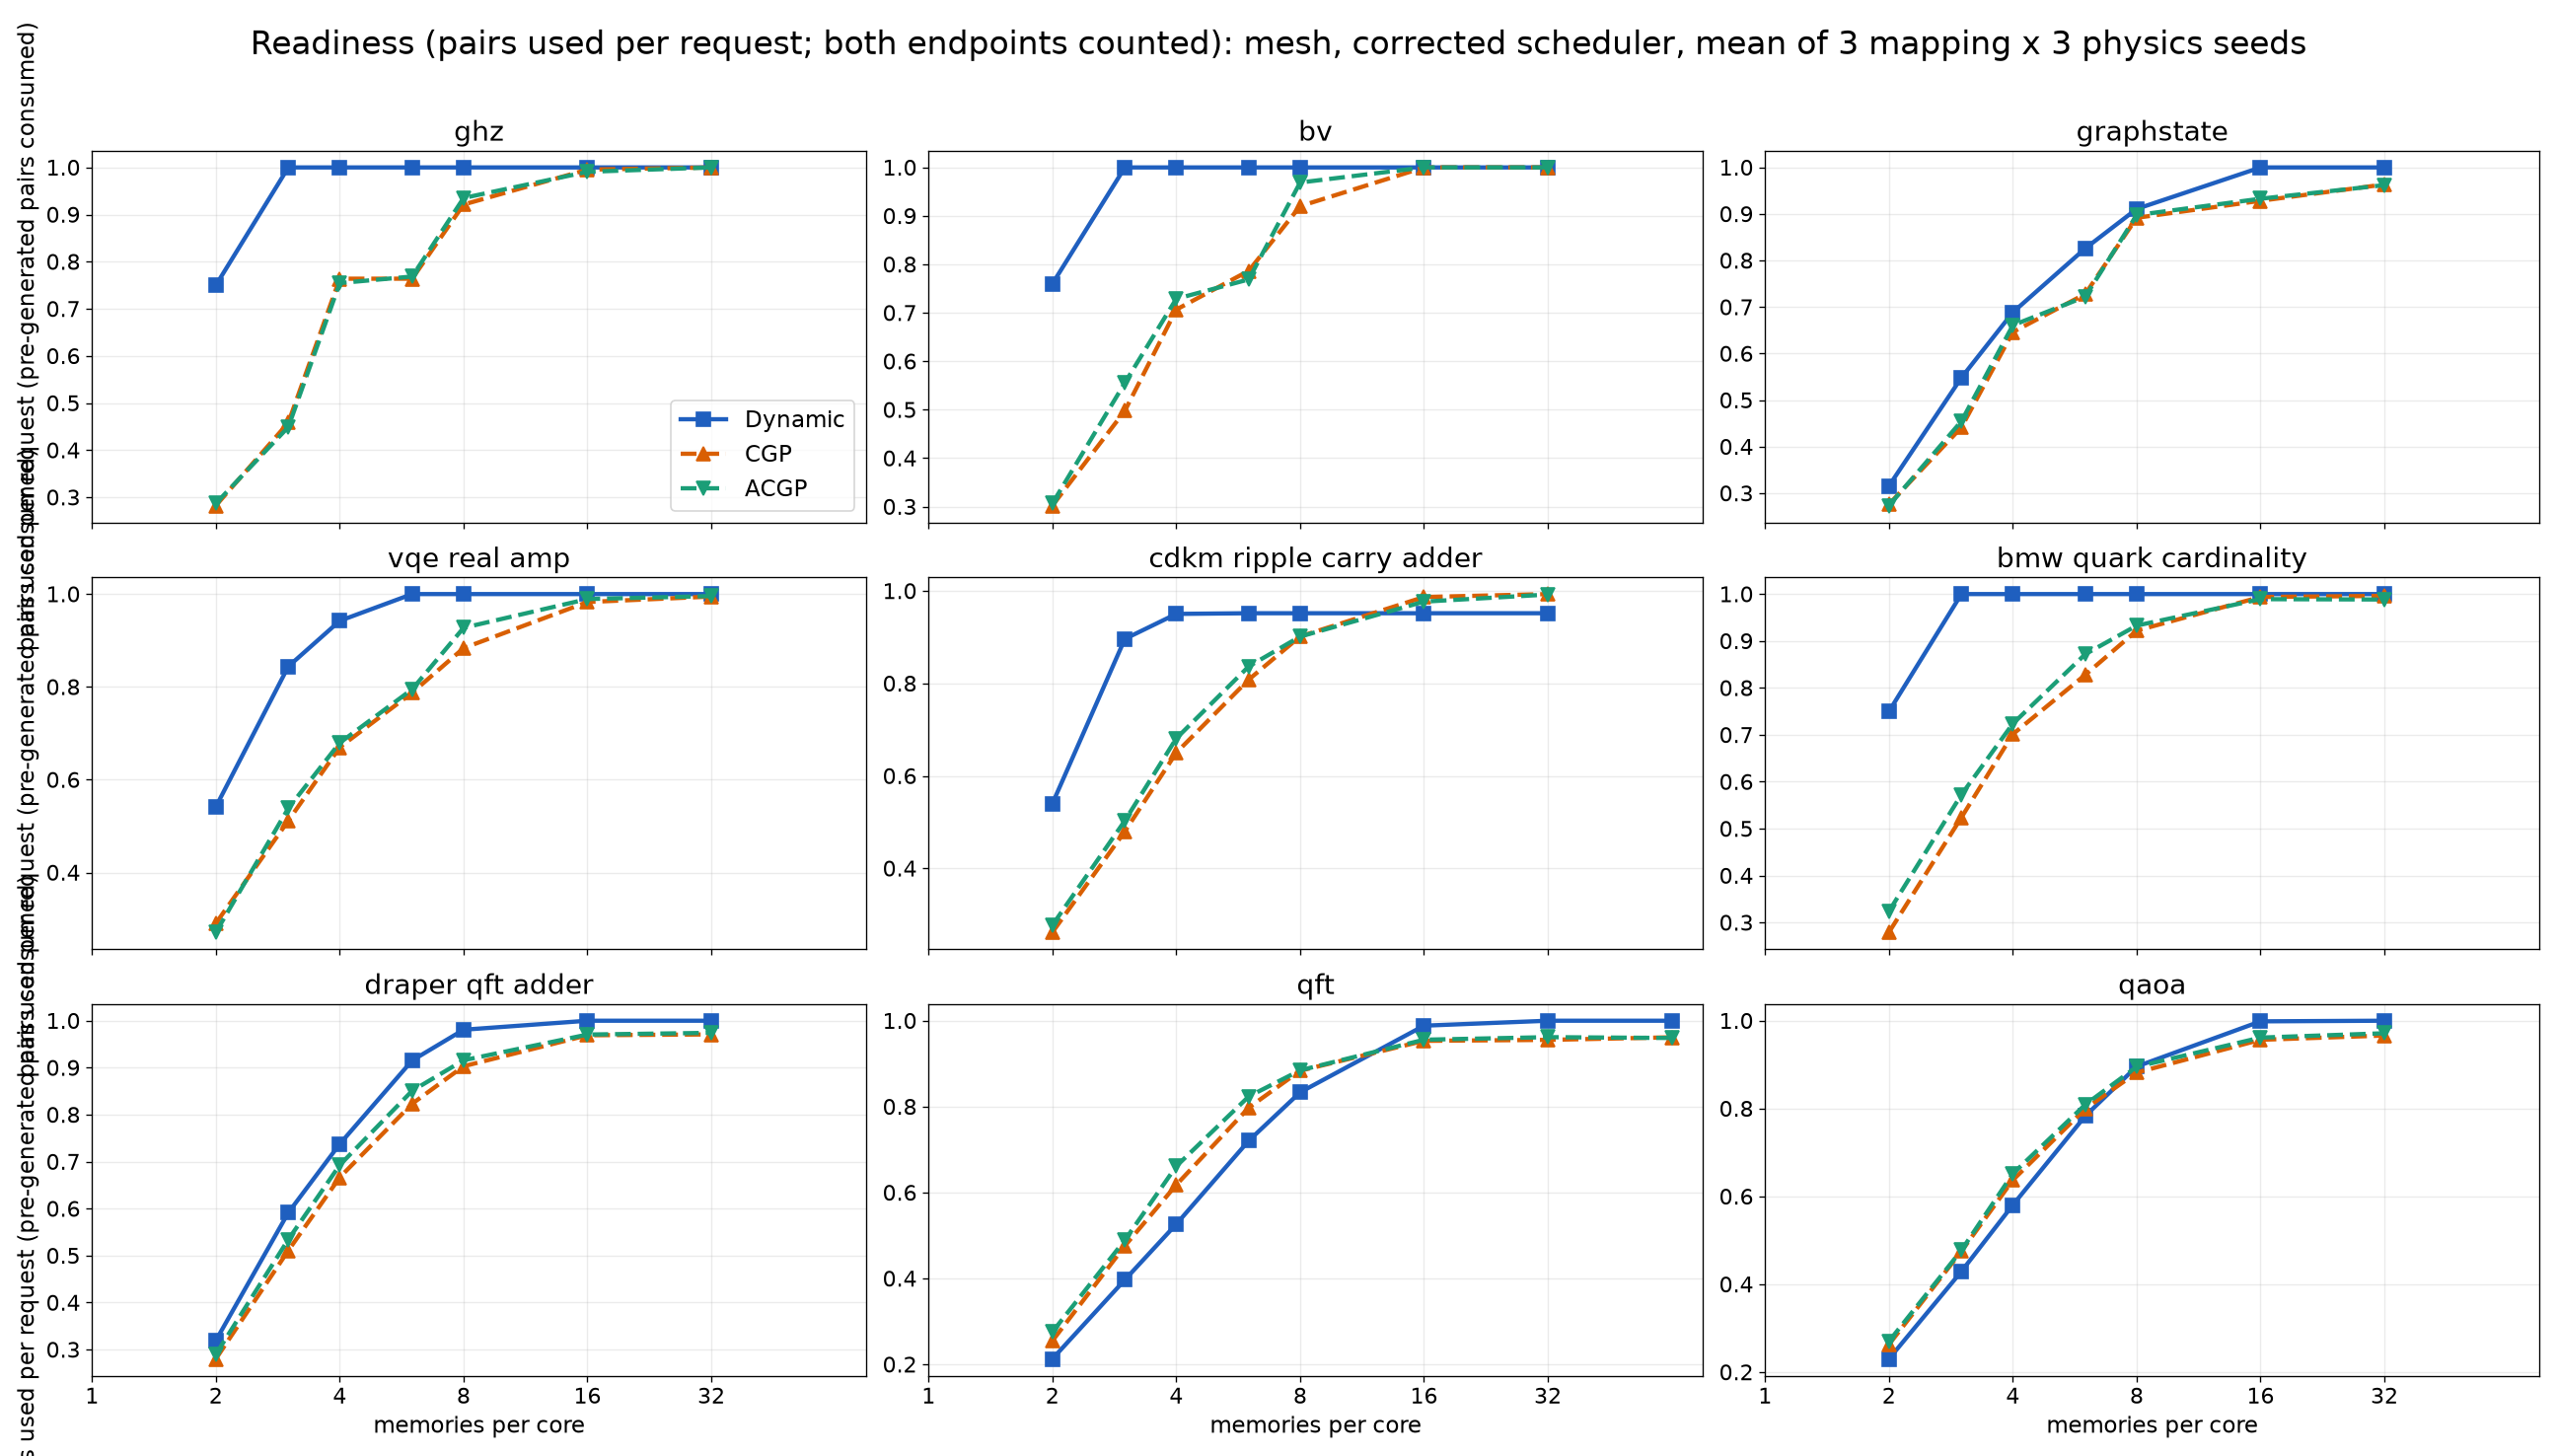
\includegraphics[width=\linewidth,height=0.80\textheight,keepaspectratio]{fp_mesh_readiness.png}
\caption{Pre-generated pairs consumed per request (pairs are counted at both endpoints, so the unit is pairs used divided by twice the requests). Mesh, corrected scheduler, mean of three mapping seeds of the mean of three physics seeds; CGP and ACGP cache at most memories$-1$ pairs per core.}
\label{fig:fp-mesh-ready}
\end{figure}
\end{landscape}

Readiness differs less than one would expect. At four memories dynamic serves $100\%$ of the requests of BMW, Bernstein--Vazirani and GHZ from a ready pair, $94$ to $95\%$ on VQE and the CDKM adder, but only $53$ to $74\%$ on the four congested circuits,
where the planner could not place a preparation for the rest within the compiler's memories (for QFT it placed $1\,330$ of $2\,510$ requests). CGP and ACGP find a cached pair for $62$ to $76\%$ of the requests at four memories --- more than dynamic on QFT and QAOA --- because a cached pair for a link serves any request
on that link, yet they are slower, because a request that has such a pair still has to wait for a memory of its own (Section~\ref{sec:code-reading}).

\section{Waiting}
\begin{landscape}
\begin{figure}[p]
\centering
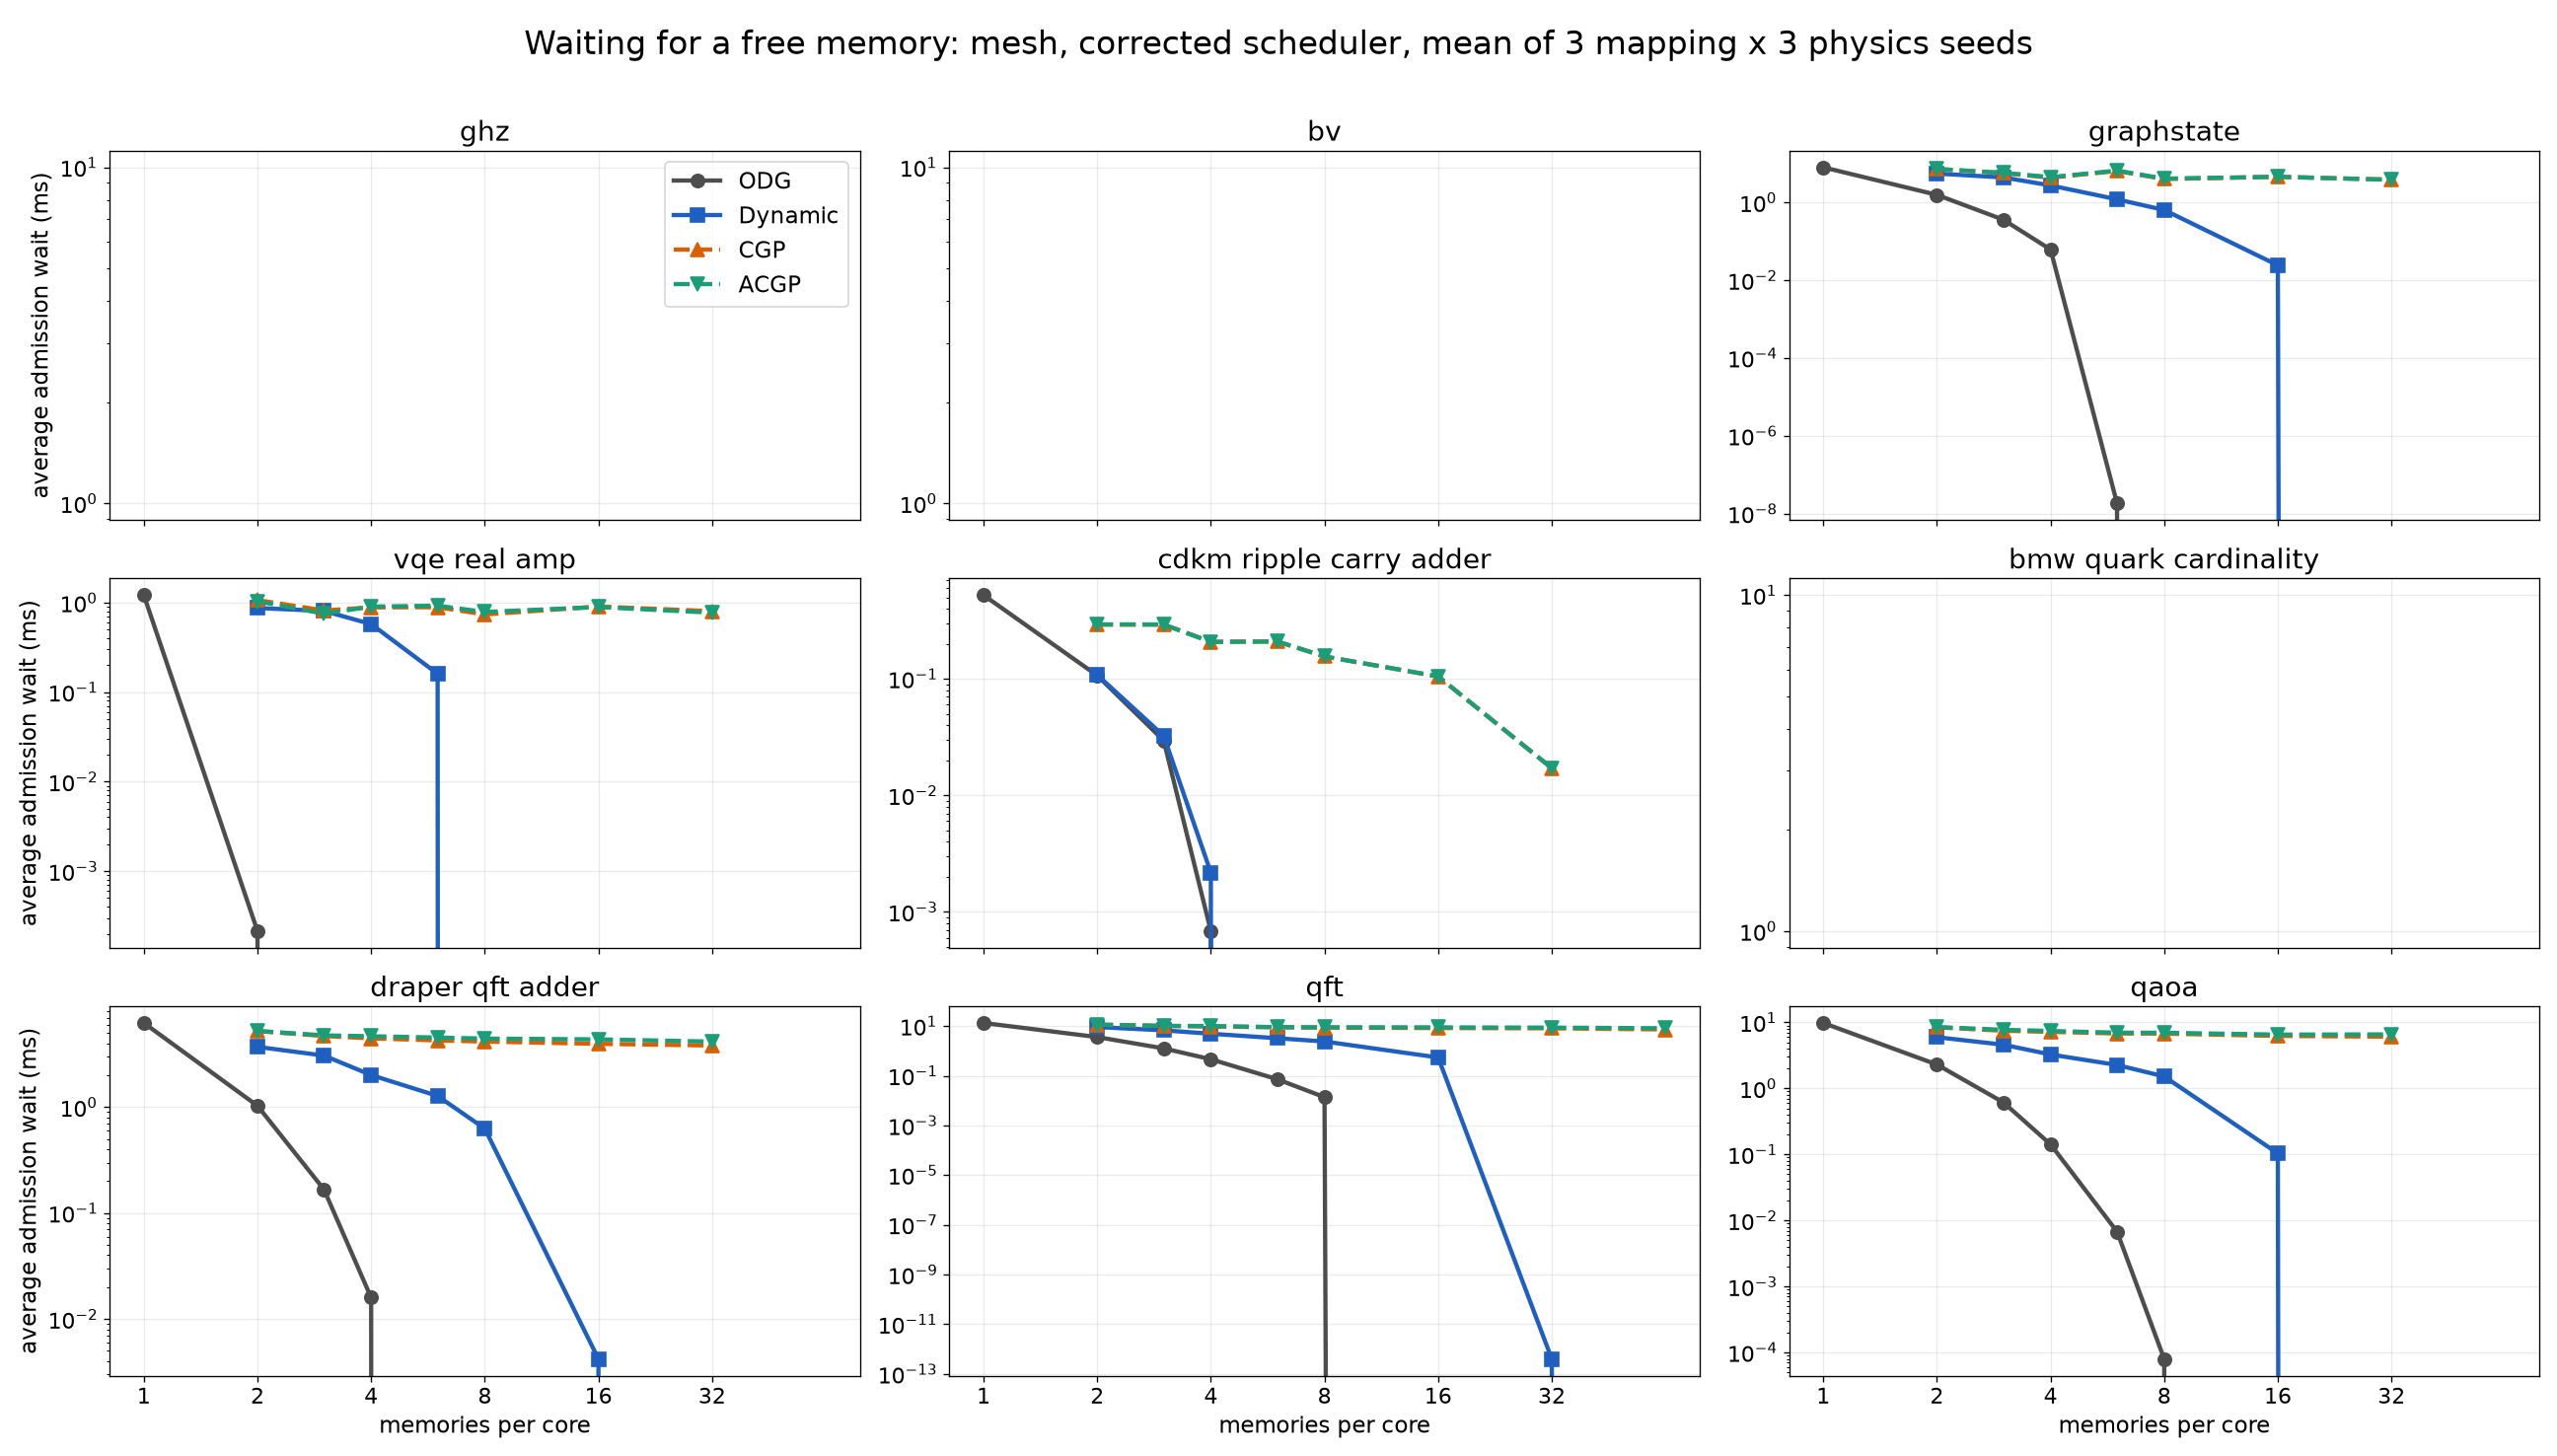
\includegraphics[width=\linewidth,height=0.80\textheight,keepaspectratio]{fp_mesh_wait.png}
\caption{Average wait for a free memory (log scale). Mesh, corrected scheduler, mean of three mapping seeds of the mean of three physics seeds; CGP and ACGP cache at most memories$-1$ pairs per core.}
\label{fig:fp-mesh-wait}
\end{figure}
\end{landscape}

\begin{table}[H]
\centering\small
\resizebox{\ifdim\width>\linewidth\linewidth\else\width\fi}{!}{%
\begin{tabular}{@{}lrrrr@{}}
\toprule
Workload & ODG & Dynamic & CGP & ACGP \\
\midrule
GHZ & 0.00 & 0.00 & 0.00 & 0.00 \\
Bernstein--Vazirani & 0.00 & 0.00 & 0.00 & 0.00 \\
BMW/QUARK cardinality & 0.00 & 0.00 & 0.00 & 0.00 \\
VQE real amplitudes & 0.00 & 0.58 & 0.88 & 0.90 \\
CDKM ripple-carry adder & 0.00 & 0.00 & 0.21 & 0.21 \\
Graph state & 0.06 & 2.73 & 4.33 & 4.46 \\
Draper QFT adder & 0.02 & 2.01 & 4.46 & 4.67 \\
QAOA & 0.14 & 3.27 & 7.20 & 7.42 \\
QFT & 0.46 & 4.91 & 9.54 & 10.06 \\
\bottomrule
\end{tabular}}
\caption{Wait for a free memory (ms), mesh, 4 memories per core (modelled), mean of three mapping seeds of the mean of three physics seeds.}
\label{tab:fp-mesh-wait-4}
\end{table}

Waiting for a free memory is where the policies differ. On the congested circuits at four memories ODG waits $0.02$ to $0.46$\,ms on average, dynamic $2.0$ to $4.9$\,ms and CGP and ACGP $4.3$ to $10.1$\,ms; on the other five circuits nobody waits
more than about a millisecond. The cause is the number of memory cards held by pre-generated pairs (Chapter~\ref{ch:why-dynamic}).

\section{The torus}
\begin{table}[H]
\centering\small
\resizebox{\ifdim\width>\linewidth\linewidth\else\width\fi}{!}{%
\begin{tabular}{@{}lrrrr@{}}
\toprule
Workload & ODG & Dynamic & CGP & ACGP \\
\midrule
GHZ & 1.15 & 0.28 & 0.72 & 0.77 \\
Bernstein--Vazirani & 1.11 & 0.23 & 0.50 & 0.43 \\
BMW/QUARK cardinality & 1.10 & 0.25 & 0.61 & 0.54 \\
VQE real amplitudes & 1.14 & 0.48 & 1.00 & 1.02 \\
CDKM ripple-carry adder & 1.09 & 0.31 & 0.74 & 0.69 \\
Graph state & 1.11 & 1.99 & 4.06 & 4.05 \\
Draper QFT adder & 1.13 & 2.71 & 5.81 & 6.01 \\
QAOA & 1.17 & 3.00 & 6.49 & 6.37 \\
QFT & 1.21 & 3.38 & 7.46 & 7.62 \\
\bottomrule
\end{tabular}}
\caption{Request latency (ms), torus, 4 memories per core (modelled), mean of three mapping seeds of the mean of three physics seeds.}
\label{tab:fp-torus-lat-4}
\end{table}

\begin{table}[H]
\centering\small
\resizebox{\ifdim\width>\linewidth\linewidth\else\width\fi}{!}{%
\begin{tabular}{@{}lrrrrrrr@{}}
\toprule
Workload & 2 & 3 & 4 & 6$^*$ & 8$^*$ & 16$^*$ & 32$^*$ \\
\midrule
GHZ & 68\% & 75\% & 75\% & 75\% & 75\% & 75\% & 75\% \\
Bernstein--Vazirani & 67\% & 79\% & 79\% & 79\% & 79\% & 79\% & 79\% \\
BMW/QUARK cardinality & 66\% & 77\% & 77\% & 77\% & 77\% & 77\% & 77\% \\
VQE real amplitudes & 43\% & 55\% & 58\% & 66\% & 74\% & 76\% & 76\% \\
CDKM ripple-carry adder & 40\% & 66\% & 72\% & 73\% & 73\% & 73\% & 73\% \\
Graph state & -98\% & -131\% & -79\% & -21\% & 44\% & 77\% & 77\% \\
Draper QFT adder & -119\% & -224\% & -141\% & -37\% & 33\% & 77\% & 77\% \\
QAOA & -110\% & -193\% & -157\% & -65\% & 2\% & 77\% & 78\% \\
QFT & -125\% & -219\% & -179\% & -85\% & -3\% & 77\% & 78\% \\
\bottomrule
\end{tabular}}
\caption{Latency gain of dynamic over on-demand, $(\text{ODG}-\text{Dyn.})/\text{ODG}$, torus; negative means dynamic is slower. Budgets marked $^*$ are counterfactual.}
\label{tab:fp-torus-gain}
\end{table}

\begin{table}[H]
\centering\small
\resizebox{\ifdim\width>\linewidth\linewidth\else\width\fi}{!}{%
\begin{tabular}{@{}lcccrrrr@{}}
\toprule
Workload & Dynamic beats ODG from (memories) & vs CGP win/tie/loss & vs ACGP win/tie/loss & Fidelity Dyn. & CGP & ACGP & ODG \\
\midrule
GHZ & 2 & 5/2/0 & 5/2/0 & 0.931 & 0.878 & 0.879 & 0.950 \\
Bernstein--Vazirani & 2 & 6/1/0 & 6/1/0 & 0.930 & 0.871 & 0.870 & 0.950 \\
BMW/QUARK cardinality & 2 & 7/0/0 & 7/0/0 & 0.931 & 0.880 & 0.879 & 0.950 \\
VQE real amplitudes & 2 & 7/0/0 & 7/0/0 & 0.929 & 0.902 & 0.906 & 0.950 \\
CDKM ripple-carry adder & 2 & 7/0/0 & 7/0/0 & 0.925 & 0.919 & 0.916 & 0.950 \\
Graph state & 8 & 7/0/0 & 7/0/0 & 0.919 & 0.894 & 0.894 & 0.950 \\
Draper QFT adder & 8 & 7/0/0 & 7/0/0 & 0.925 & 0.910 & 0.908 & 0.950 \\
QAOA & 8 & 7/0/0 & 7/0/0 & 0.925 & 0.906 & 0.906 & 0.950 \\
QFT & 16 & 8/0/0 & 8/0/0 & 0.928 & 0.910 & 0.909 & 0.950 \\
\bottomrule
\end{tabular}}
\caption{Where dynamic lies, torus. Column~2: the smallest memory count from which dynamic has lower latency than on-demand ($^\dagger$: with at least one later count where it does not). Columns~3--4: over the memory counts run for both policies (2 to 32; QFT also 64), the number at which dynamic has lower latency, equal latency (the floor reached when nothing waits) or higher latency than CGP and than ACGP. Columns~5--8: delivered fidelity at four memories.}
\label{tab:fp-torus-where}
\end{table}

\begin{table}[H]
\centering\small
\resizebox{\ifdim\width>\linewidth\linewidth\else\width\fi}{!}{%
\begin{tabular}{@{}rrrrr@{}}
\toprule
Mem. & ODG & Dynamic & CGP & ACGP \\
\midrule
1 & 9 & 0 & 0 & 0 \\
2 & 4 & 5 & 0 & 0 \\
3 & 4 & 5 & 0 & 0 \\
4 & 4 & 5 & 0 & 0 \\
6 & 4 & 5 & 0 & 0 \\
8 & 1 & 8 & 0 & 0 \\
16 & 0 & 8 & 0 & 1 \\
32 & 0 & 7 & 0 & 2 \\
\bottomrule
\end{tabular}}
\caption{Torus: number of benchmarks (of ten) on which each policy has the lowest latency at each memory count (a policy is counted only where it was run; dynamic, CGP and ACGP start at two memories).}
\label{tab:fp-torus-best}
\end{table}

The ordering is the same on the torus: dynamic is faster than the better of CGP and ACGP on every benchmark at every memory count except ties at the floor (Table~\ref{tab:fp-torus-where}); against ODG it wins on the same five benchmarks at four memories,
loses on QFT, QAOA, Draper and graph state at two to four, and overtakes ODG from eight memories on Draper, graph state and QAOA and from sixteen on QFT. CGP and ACGP beat ODG on BMW, Bernstein--Vazirani, GHZ and the CDKM adder at every
memory count and on VQE from three or four, and never on the other four. Waste is higher on the torus ($34$ to $92\%$ at four memories). The figures for the torus follow.
\clearpage\newgeometry{margin=12mm}\begin{landscape}
\begin{figure}[p]
\centering
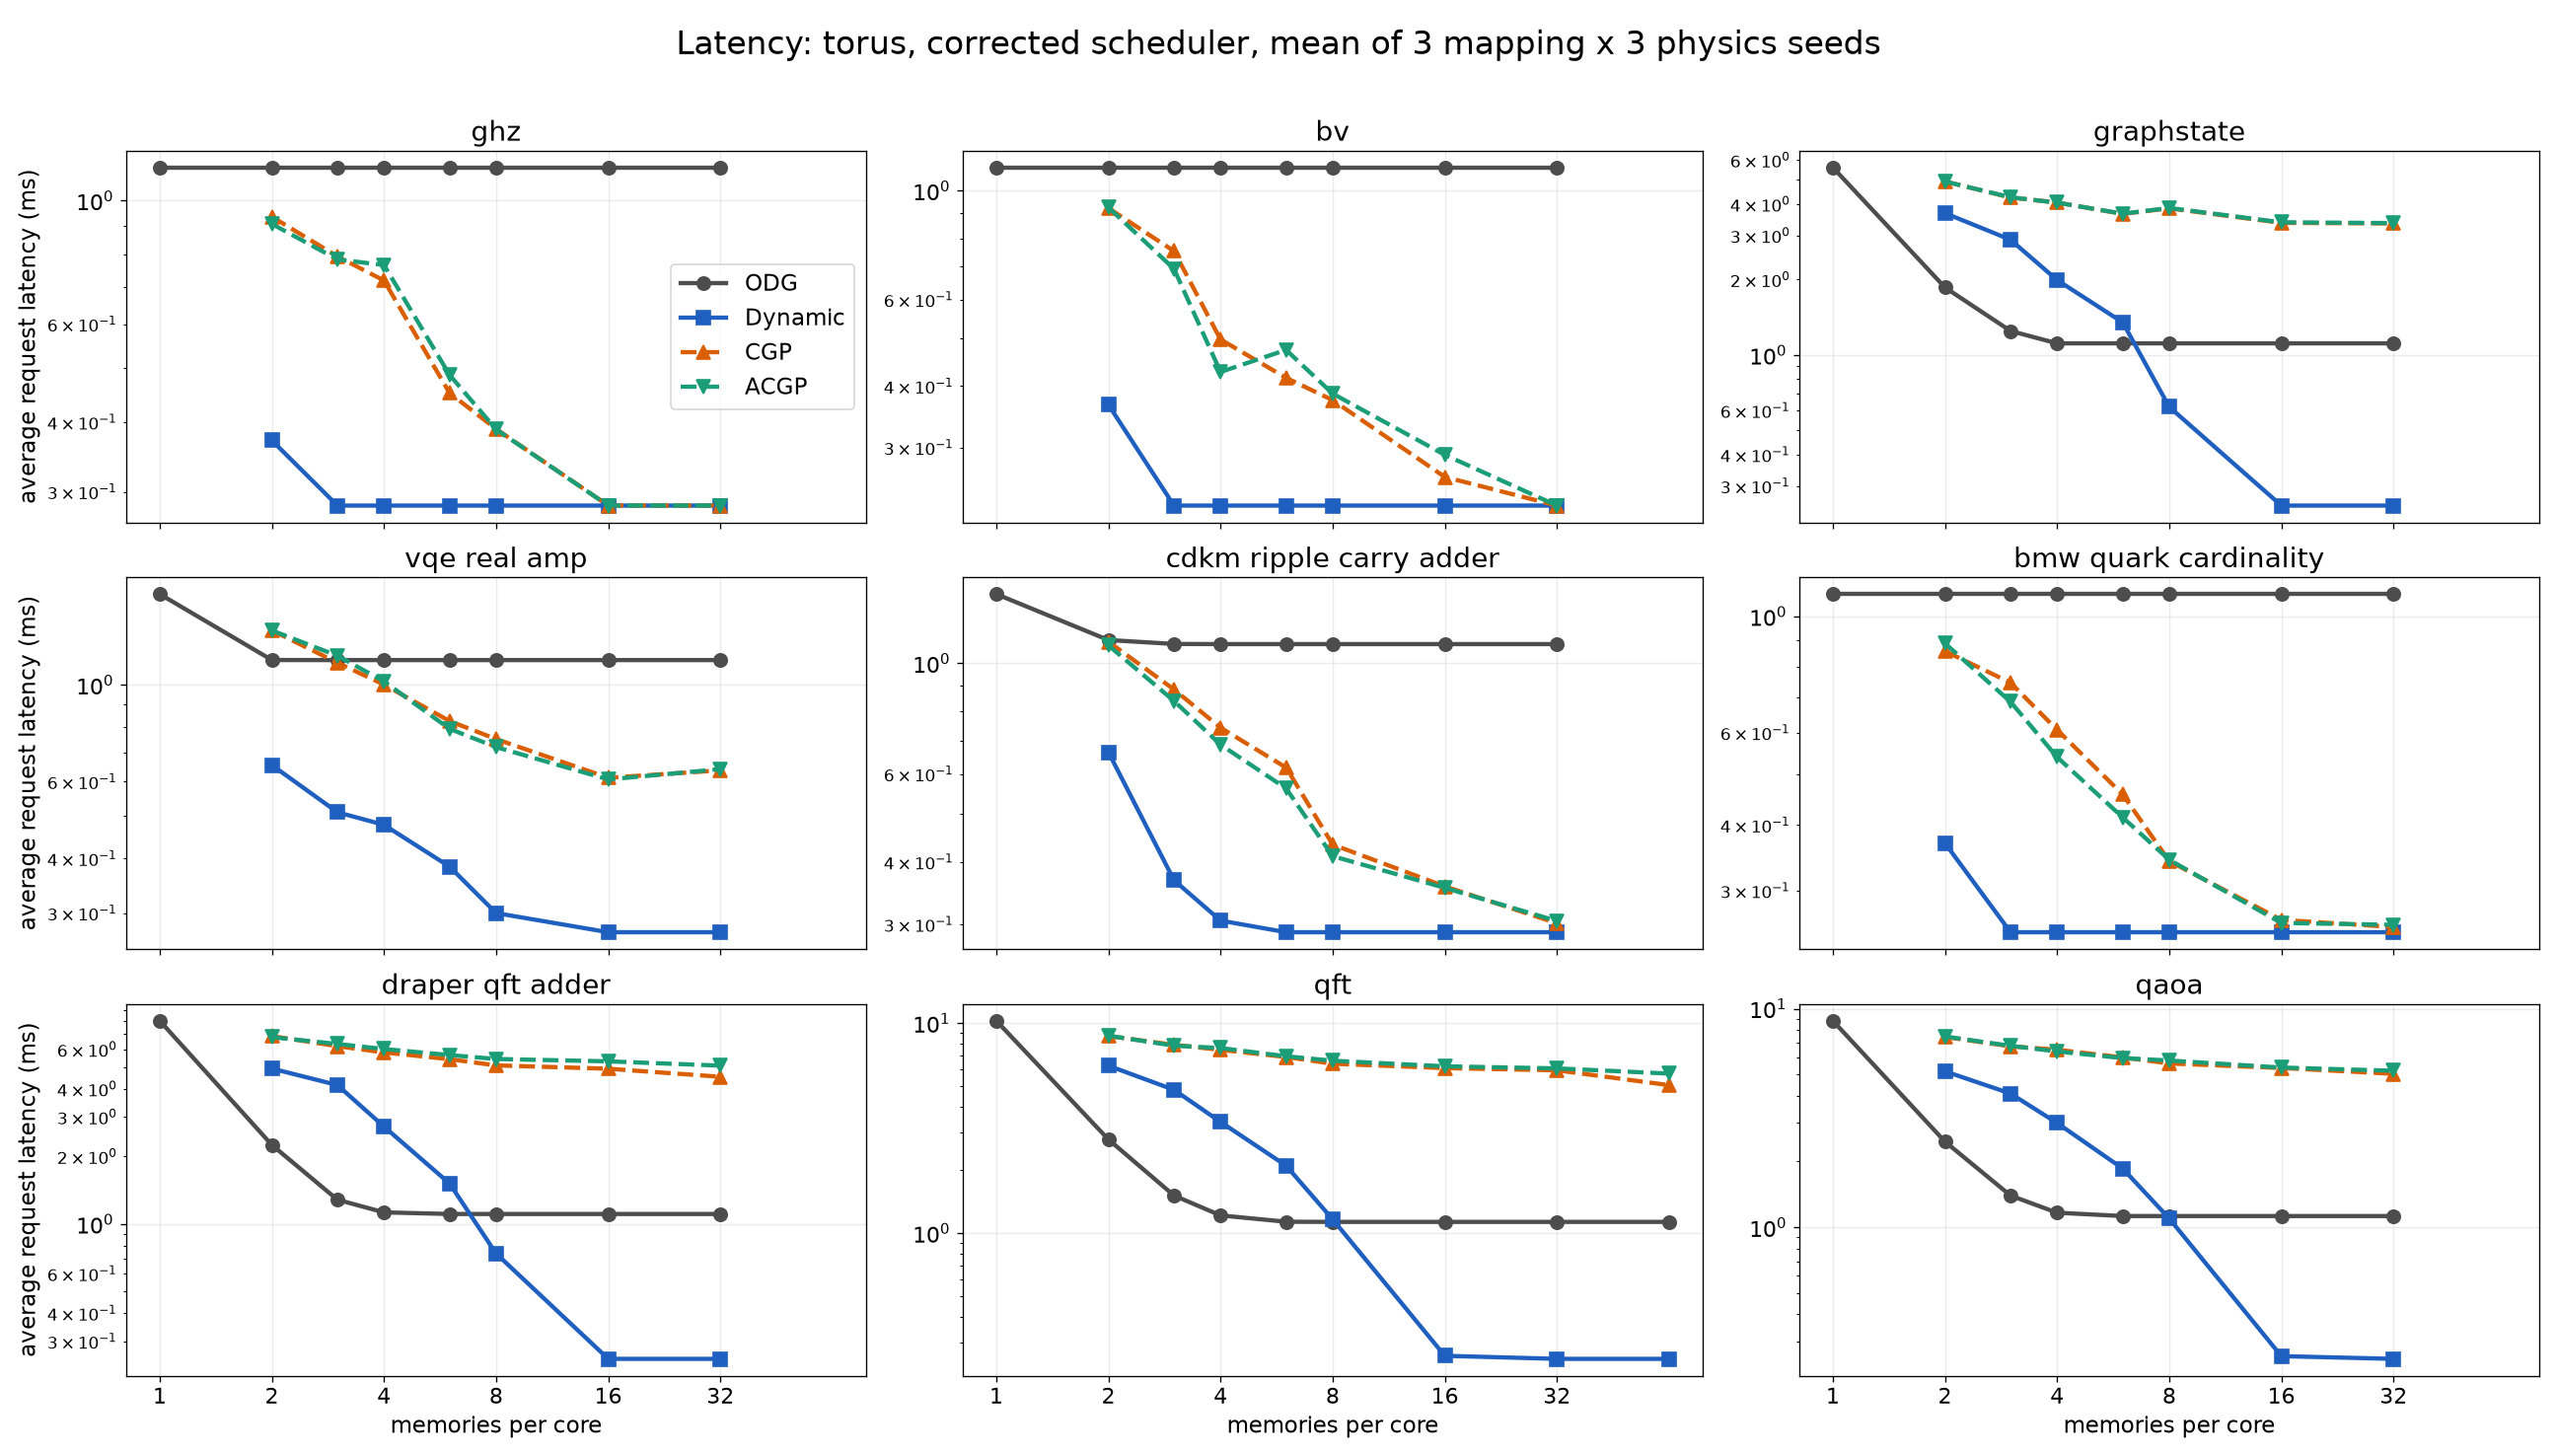
\includegraphics[width=\linewidth,height=0.82\textheight,keepaspectratio]{fp_torus_latency.png}
\caption{Request latency against memories per core, all four policies (log scale). Torus, corrected scheduler, mean of three mapping seeds of the mean of three physics seeds; CGP and ACGP cache at most memories$-1$ pairs per core.}
\label{fig:fp-torus-lat}
\end{figure}
\end{landscape}\clearpage\restoregeometry

\clearpage\newgeometry{margin=12mm}\begin{landscape}
\begin{figure}[p]
\centering
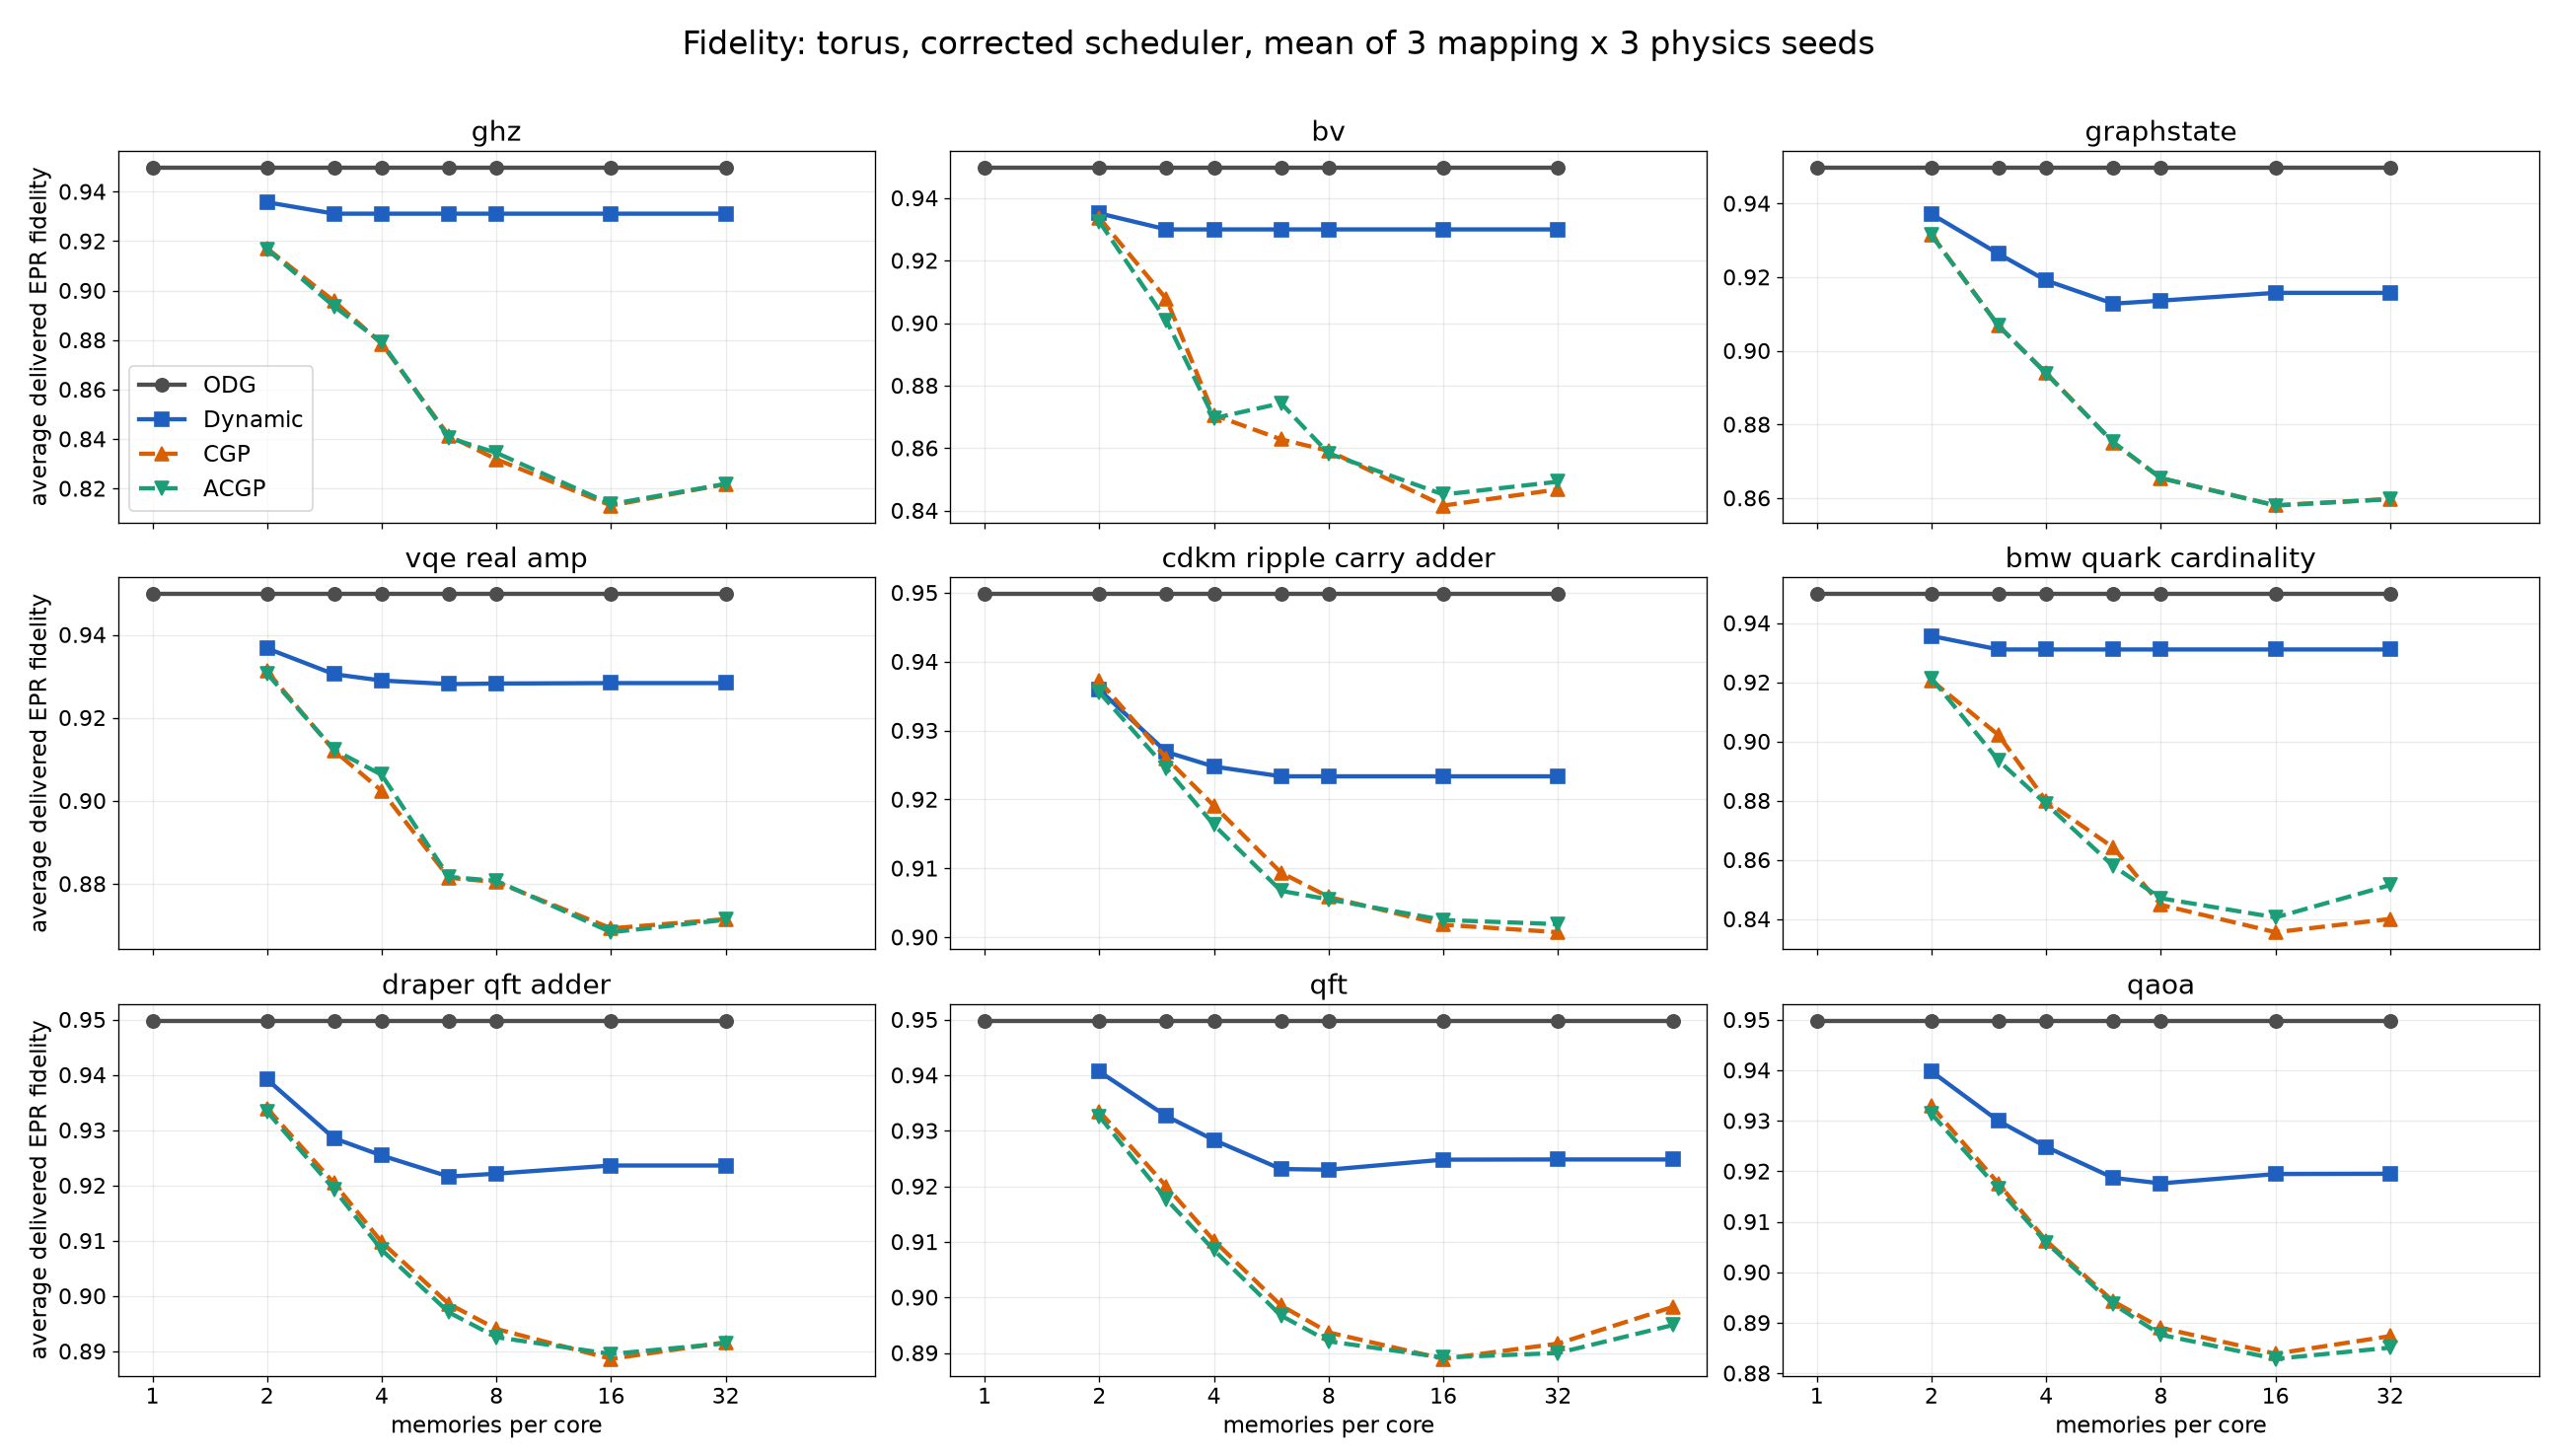
\includegraphics[width=\linewidth,height=0.82\textheight,keepaspectratio]{fp_torus_fidelity.png}
\caption{Delivered EPR fidelity against memories per core. Torus, corrected scheduler, mean of three mapping seeds of the mean of three physics seeds; CGP and ACGP cache at most memories$-1$ pairs per core.}
\label{fig:fp-torus-fid}
\end{figure}
\end{landscape}\clearpage\restoregeometry

\clearpage\newgeometry{margin=12mm}\begin{landscape}
\begin{figure}[p]
\centering
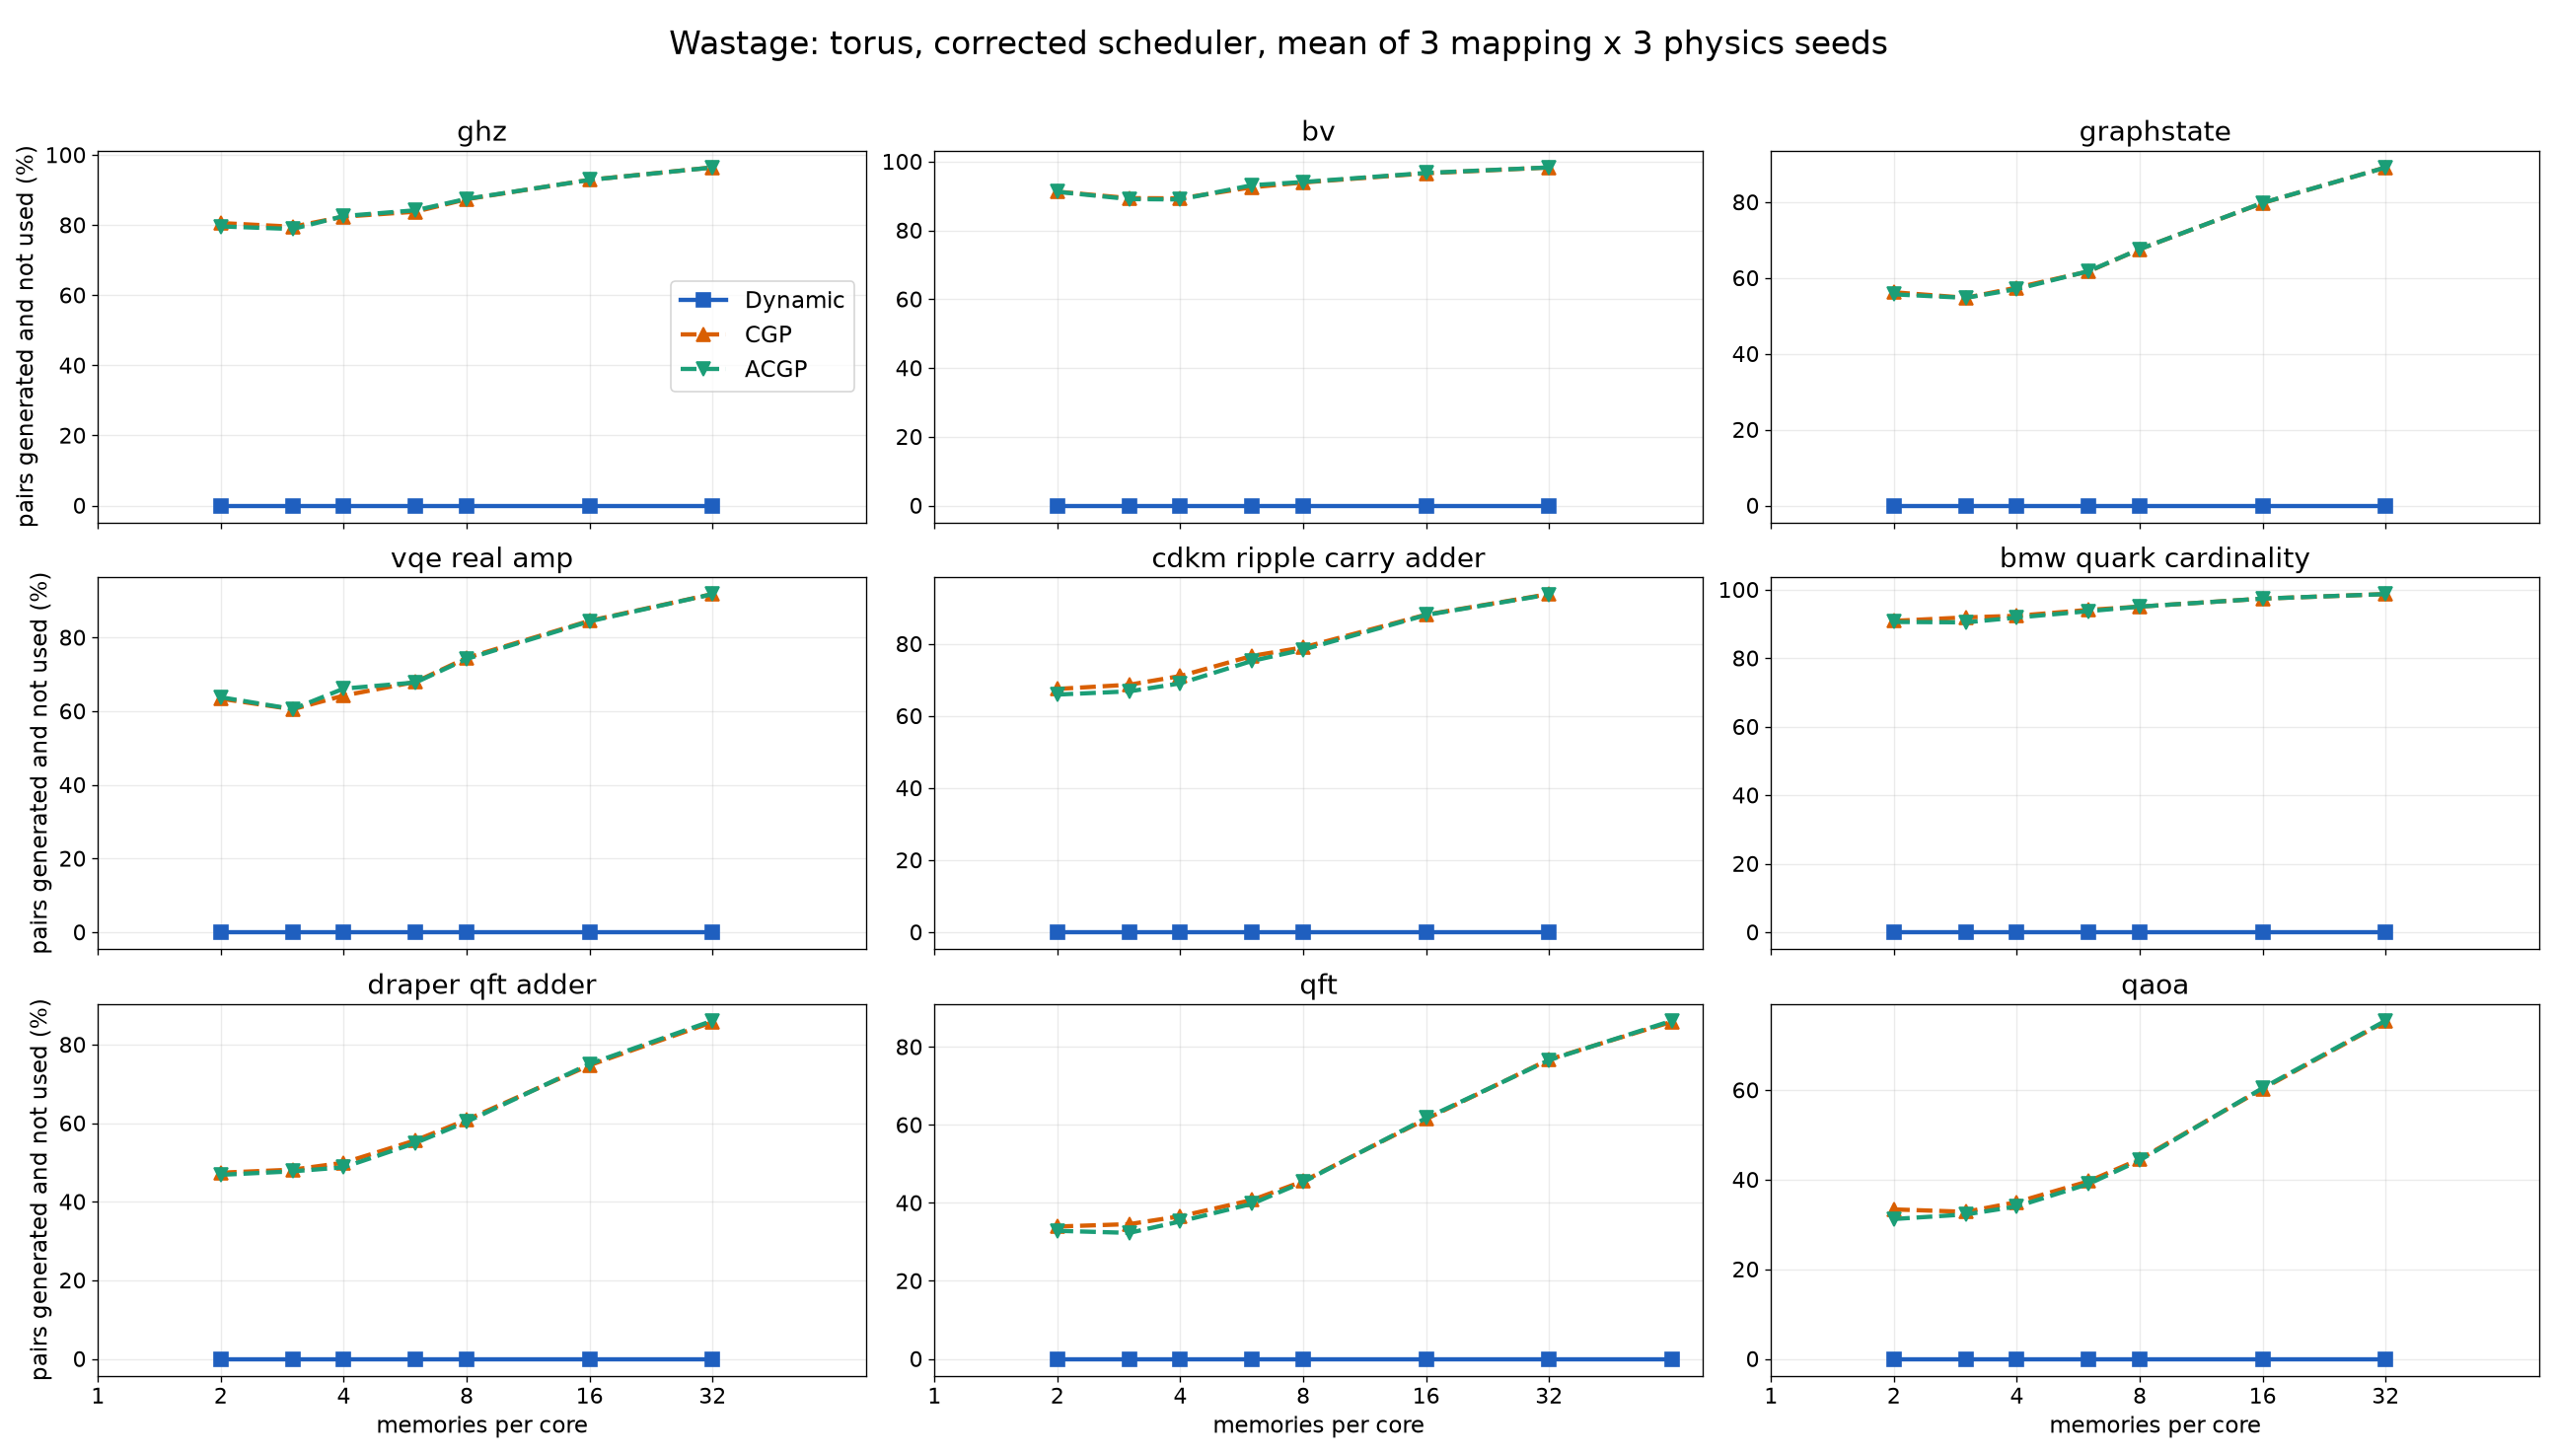
\includegraphics[width=\linewidth,height=0.82\textheight,keepaspectratio]{fp_torus_waste.png}
\caption{Pairs generated and not used by the end of the run, as a percentage of pairs generated (dynamic, CGP, ACGP). Torus, corrected scheduler, mean of three mapping seeds of the mean of three physics seeds; CGP and ACGP cache at most memories$-1$ pairs per core.}
\label{fig:fp-torus-waste}
\end{figure}
\end{landscape}\clearpage\restoregeometry

\clearpage\newgeometry{margin=12mm}\begin{landscape}
\begin{figure}[p]
\centering
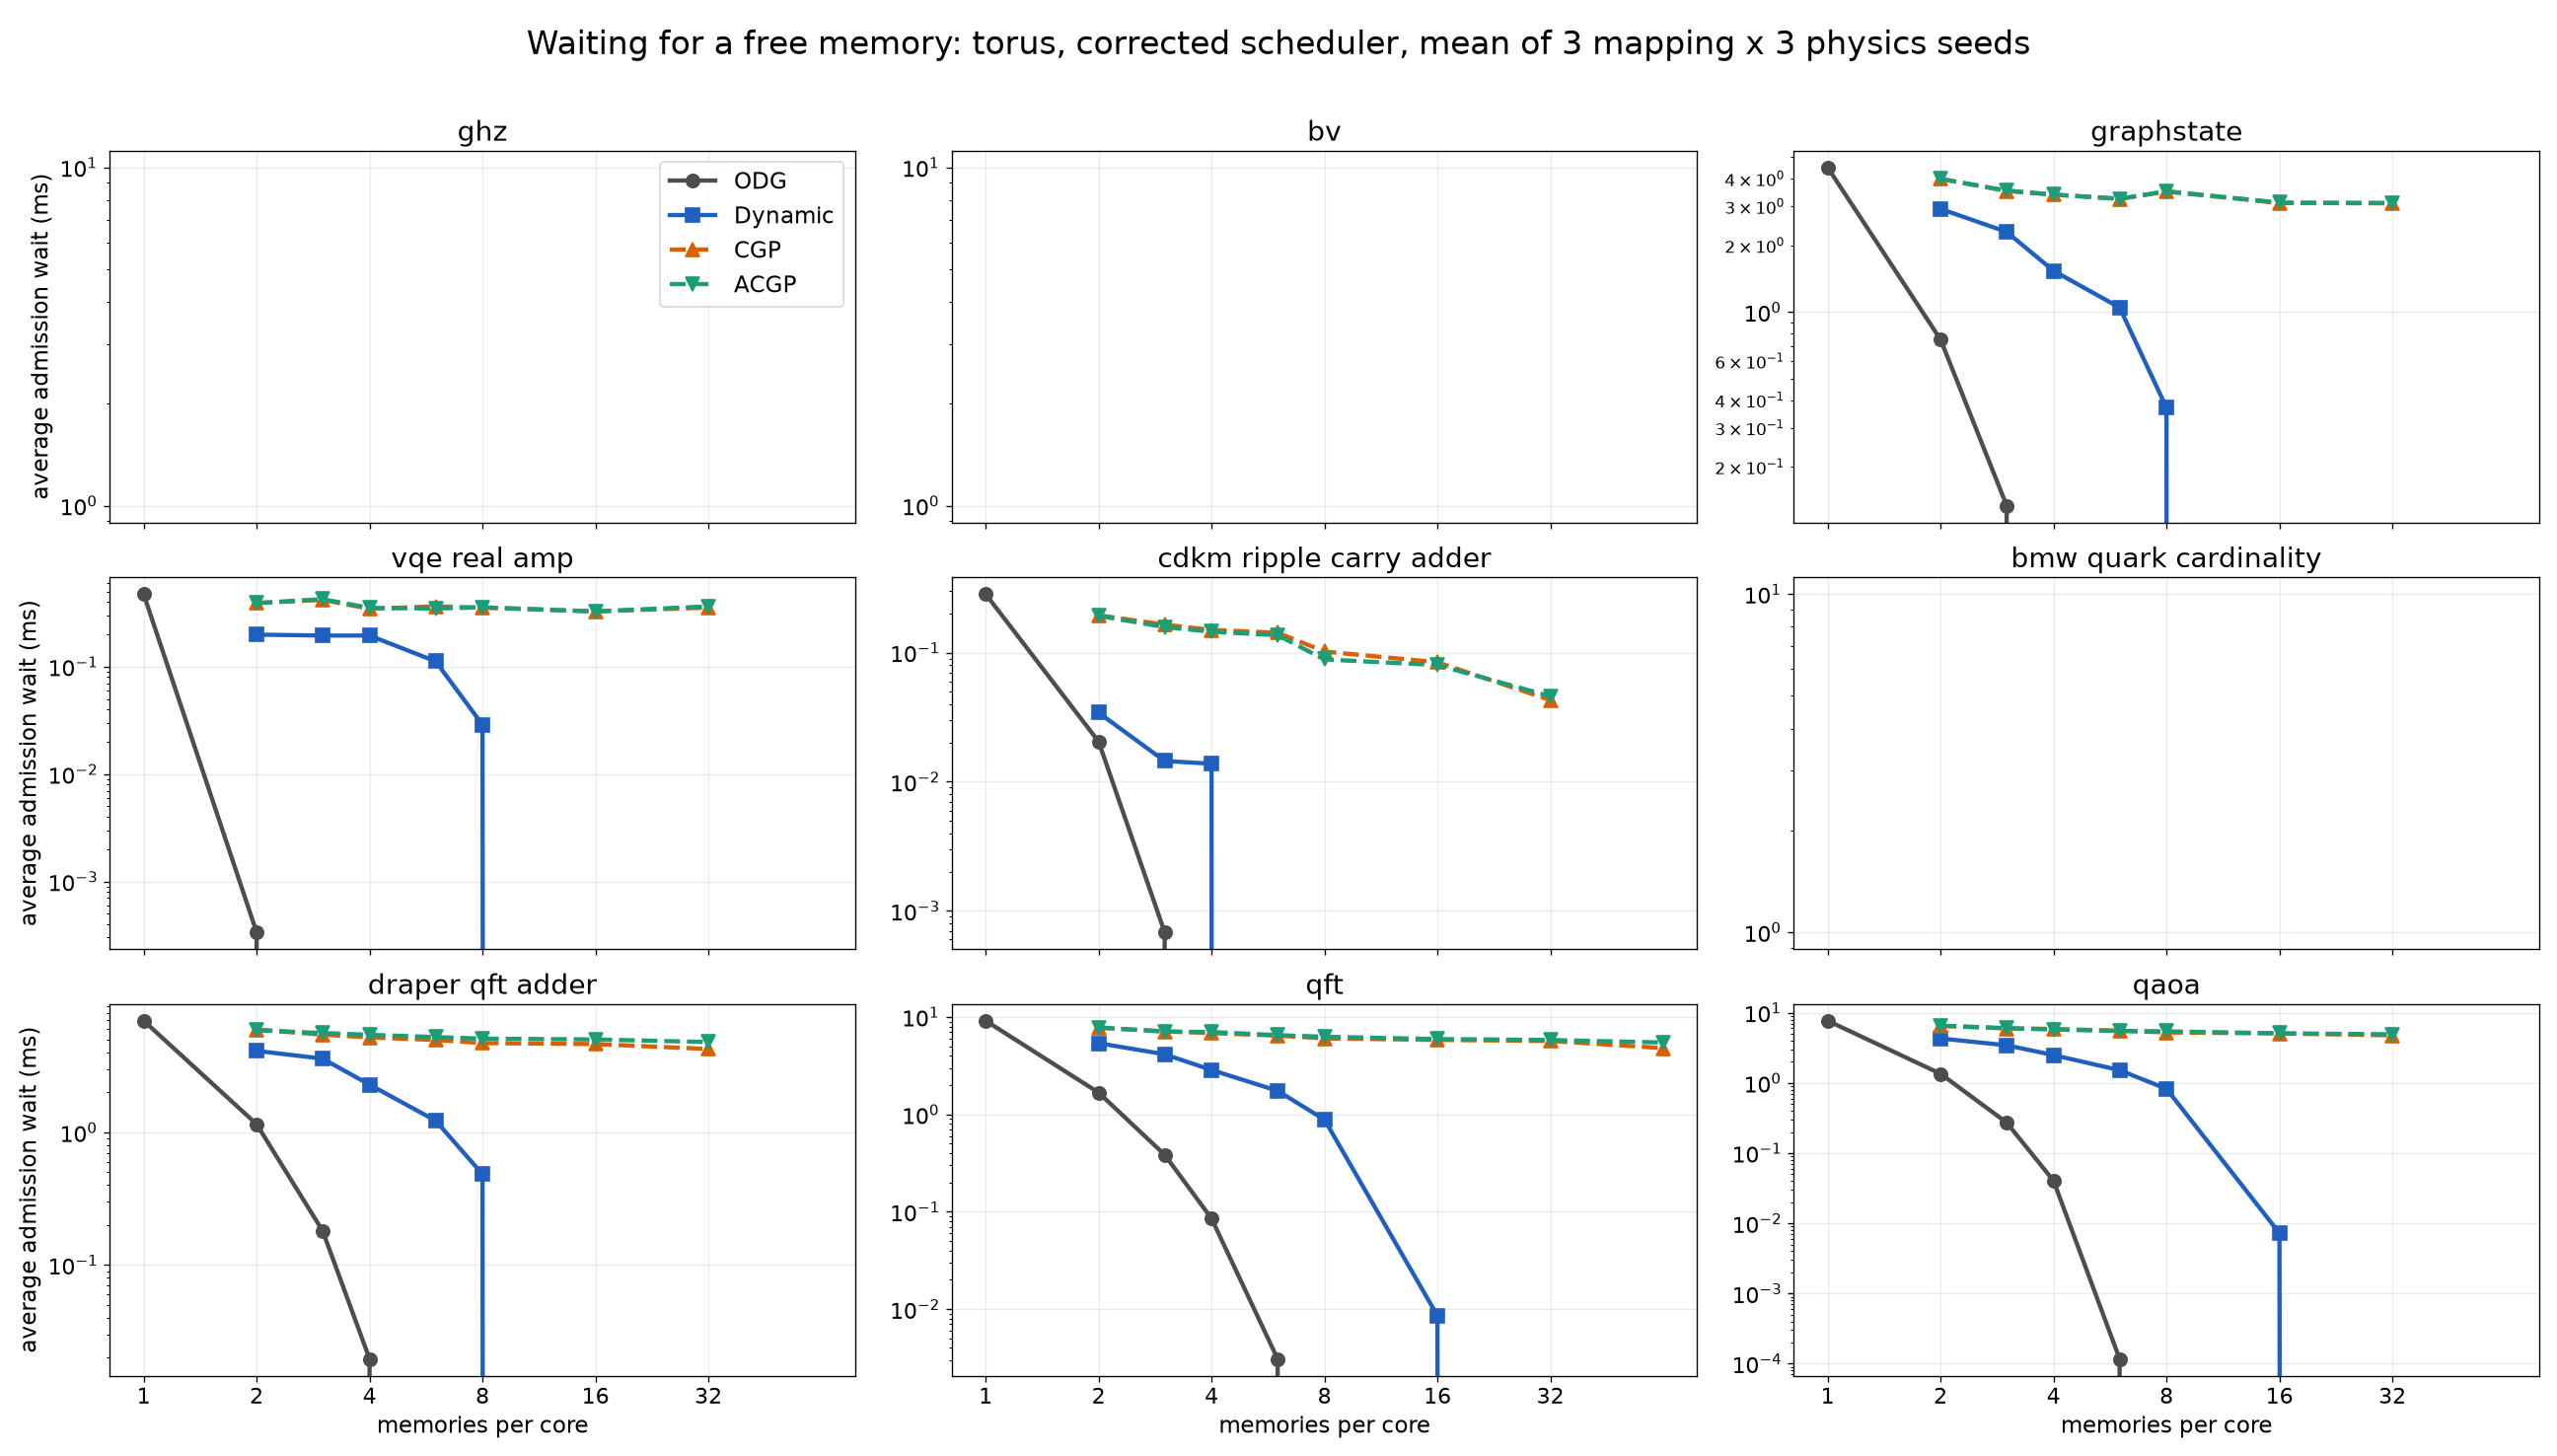
\includegraphics[width=\linewidth,height=0.82\textheight,keepaspectratio]{fp_torus_wait.png}
\caption{Average wait for a free memory (log scale). Torus, corrected scheduler, mean of three mapping seeds of the mean of three physics seeds; CGP and ACGP cache at most memories$-1$ pairs per core.}
\label{fig:fp-torus-wait}
\end{figure}
\end{landscape}\clearpage\restoregeometry

\clearpage\newgeometry{margin=12mm}\begin{landscape}
\begin{figure}[p]
\centering
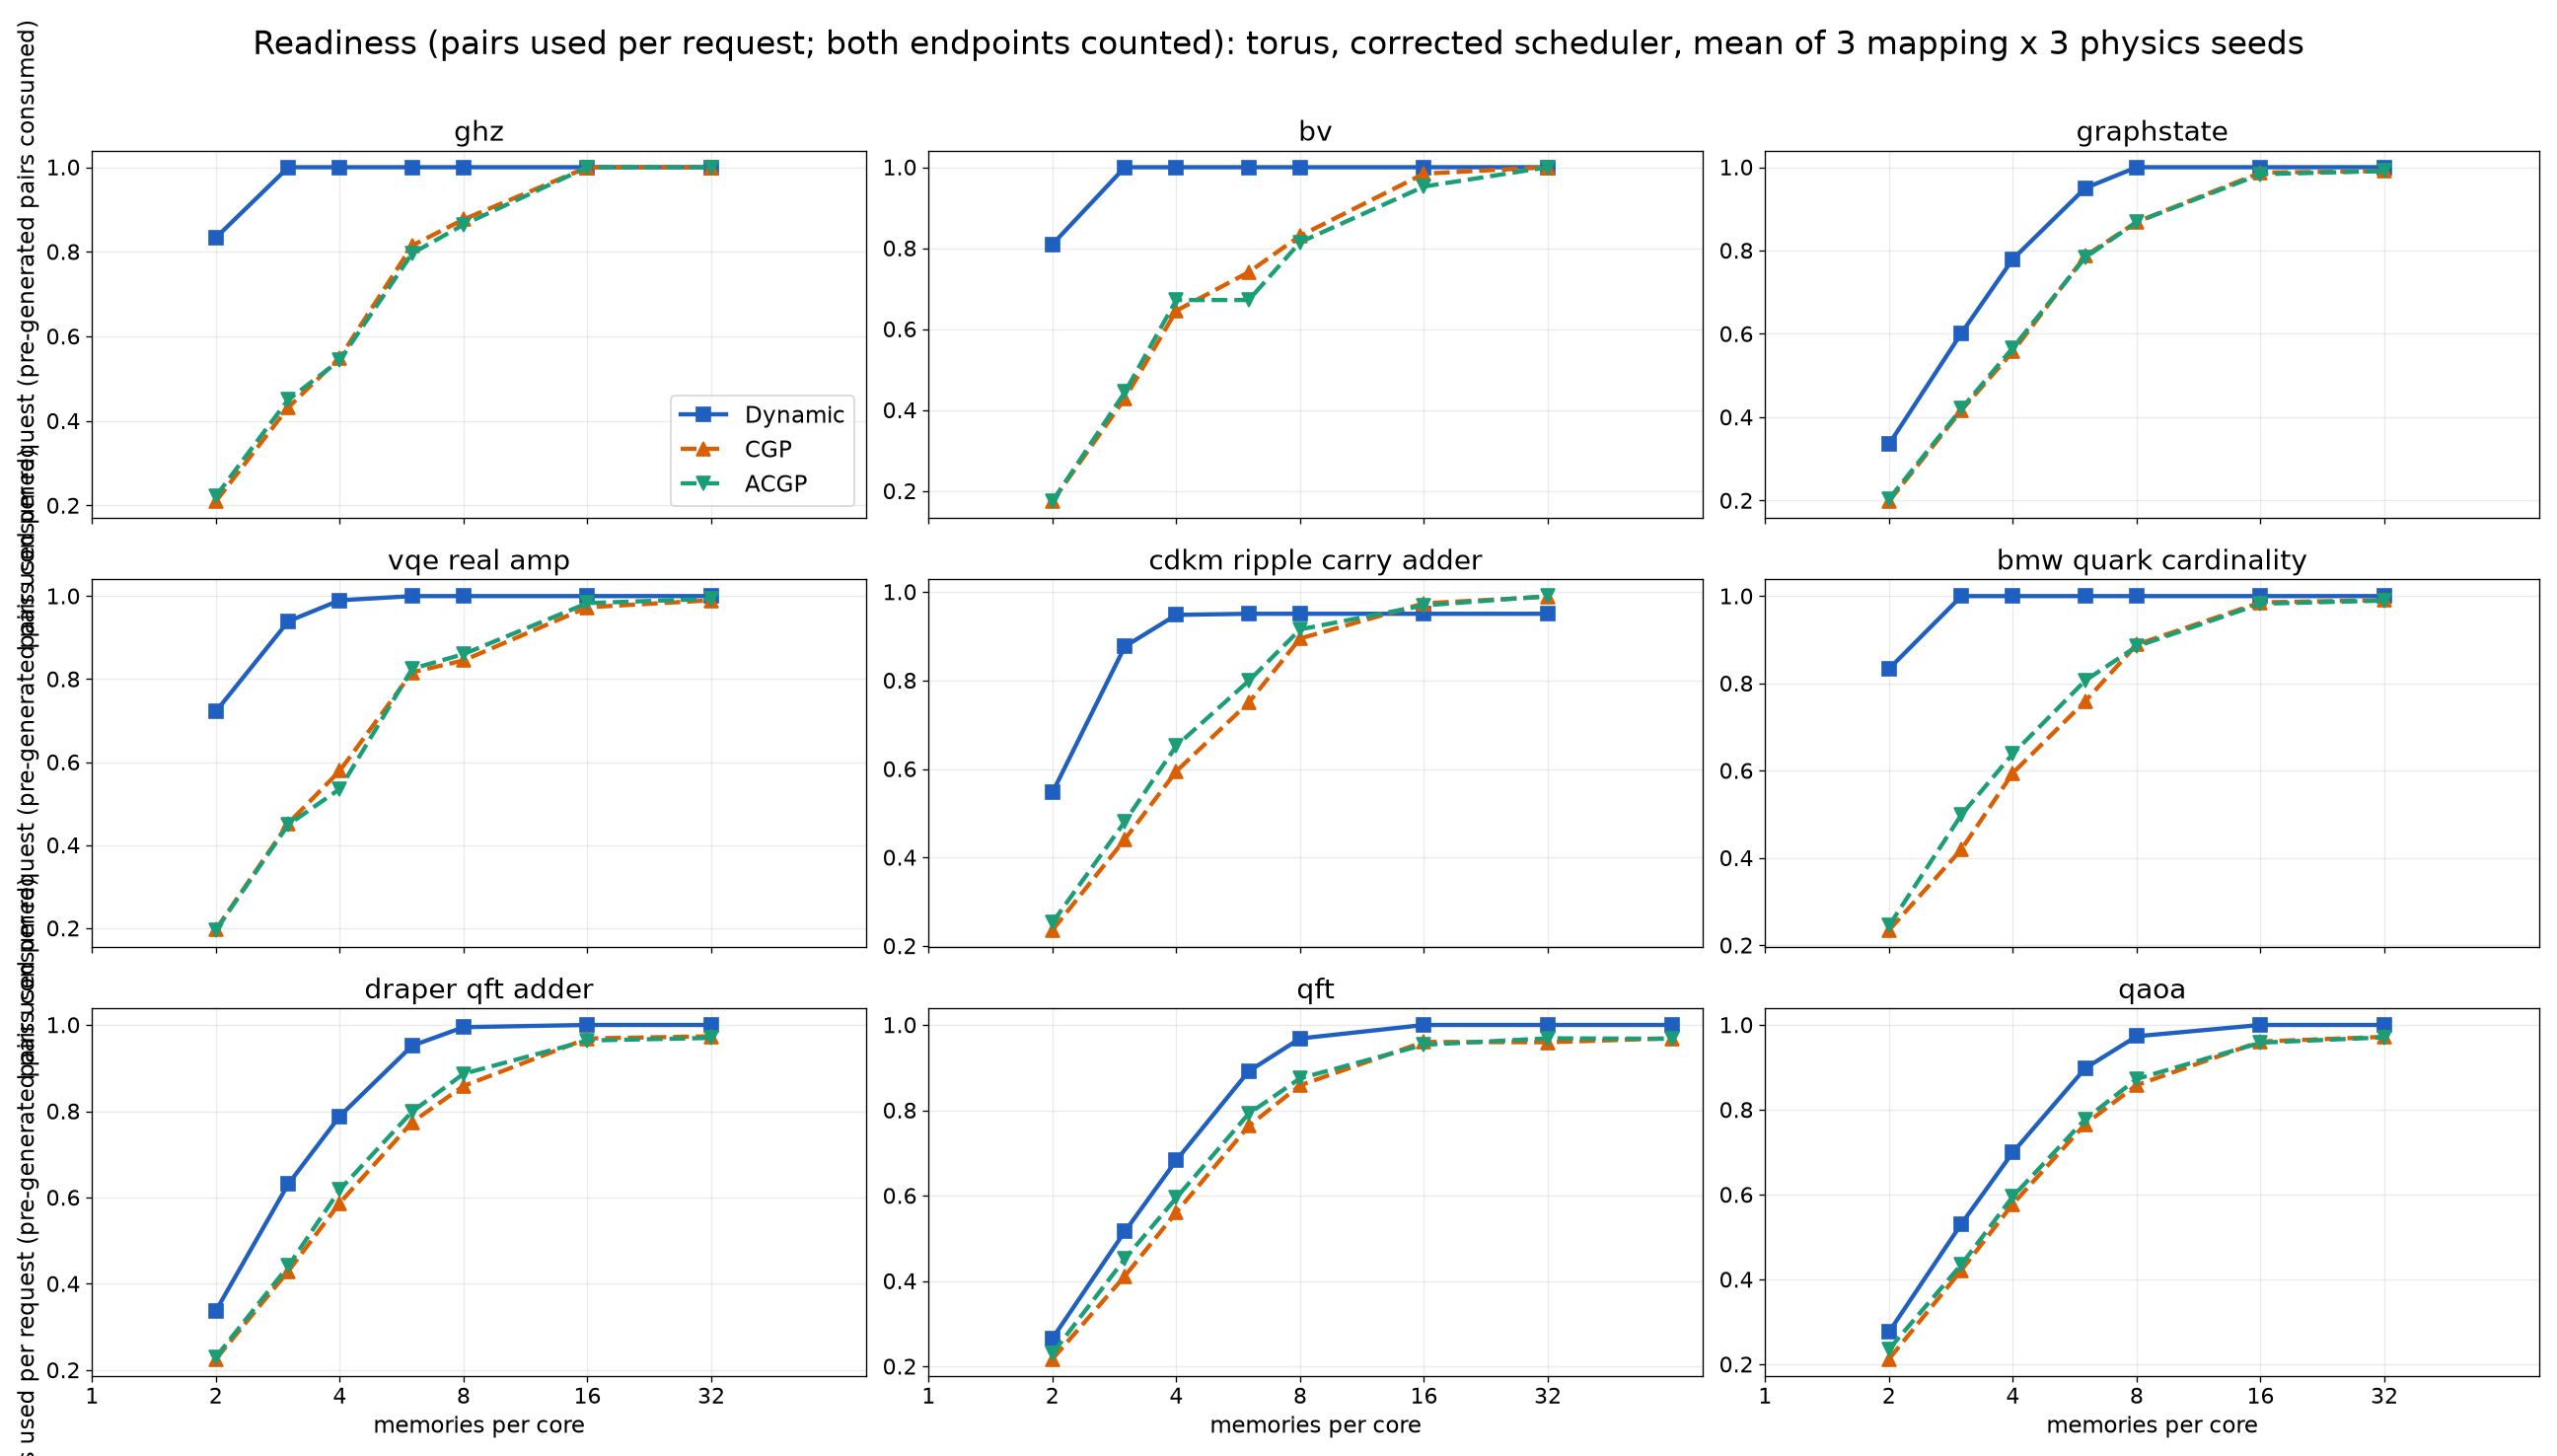
\includegraphics[width=\linewidth,height=0.82\textheight,keepaspectratio]{fp_torus_readiness.png}
\caption{Pre-generated pairs consumed per request (pairs are counted at both endpoints, so the unit is pairs used divided by twice the requests). Torus, corrected scheduler, mean of three mapping seeds of the mean of three physics seeds; CGP and ACGP cache at most memories$-1$ pairs per core.}
\label{fig:fp-torus-ready}
\end{figure}
\end{landscape}\clearpage\restoregeometry


\section{Where dynamic lies}
\begin{itemize}
  \item \textbf{Against the autonomous protocols (the stated goal): yes.} At every modelled memory count (two to four) dynamic has lower latency than CGP and ACGP on every one of the nine benchmarks, wastes none of its pairs against $34$ to $89\%$,
    and delivers higher fidelity on every benchmark ($0.916$ to $0.927$ against $0.865$ to $0.913$ at four memories). This holds on the mesh and on the torus.
  \item \textbf{Against on-demand generation: only partly.} Dynamic matches or beats ODG's latency on the benchmarks where requests rarely compete for memory (five of nine at four memories), and on all of them once the memory count reaches eight to sixteen. On the
    congested benchmarks at the modelled two to four memories it is slower than ODG, by a factor of $2.0$ to $3.5$ on the mesh and $1.8$ to $3.2$ on the torus, because prepared pairs occupy memory that requests need. It never matches ODG's fidelity.
  \item \textbf{What would change this} is not established here. The plan does not account for the memory a ready pair's own request also needs, nor for when a chain hop becomes eligible (Chapter~\ref{ch:why-dynamic}); a planner that did is a possible
    direction, not a result.
\end{itemize}
\paragraph{Limits.} Nine benchmarks (the random circuit was not run for CGP and ACGP); three mapping seeds; ACE's physical parameters, which are undecided (Appendix~\ref{app:params}); the autonomous protocols are configured with a cache cap of memories$-1$, which is my choice for fairness
and is not ACE's default; the waste of the autonomous protocols depends on the length of the workload and is only comparable within a benchmark.
